%%%%%%%%%%%%%%%%%%%%%%%%%%%%%%%%%%%%%%%%%
% Formal Book Title Page
% LaTeX Template
% Version 2.0 (23/7/17)
%
% This template was downloaded from:
% http://www.LaTeXTemplates.com
%
% Original author:
% Peter Wilson (herries.press@earthlink.net) with modifications by:
% Vel (vel@latextemplates.com)
%
% License:
% CC BY-NC-SA 3.0 (http://creativecommons.org/licenses/by-nc-sa/3.0/)
% 
% This template can be used in one of two ways:
%
% 1) Content can be added at the end of this file just before the \end{document}
% to use this title page as the starting point for your document.
%
% 2) Alternatively, if you already have a document which you wish to add this
% title page to, copy everything between the \begin{document} and
% \end{document} and paste it where you would like the title page in your
% document. You will then need to insert the packages and document 
% configurations into your document carefully making sure you are not loading
% the same package twice and that there are no clashes.
%
%%%%%%%%%%%%%%%%%%%%%%%%%%%%%%%%%%%%%%%%%

%----------------------------------------------------------------------------------------
%	PACKAGES AND OTHER DOCUMENT CONFIGURATIONS
%----------------------------------------------------------------------------------------

\documentclass[a4paper, 11pt, oneside]{article} % A4 paper size, default 11pt font size and oneside for equal margins

\newcommand{\plogo}{\fbox{$\mathcal{PL}$}} % Generic dummy publisher logo

\usepackage[utf8]{inputenc} % Required for inputting international characters
\usepackage[T1]{fontenc} % Output font encoding for international characters
\usepackage{fouriernc} % Use the New Century Schoolbook font
\usepackage{graphicx} 
\usepackage[hmarginratio=1:1,top=25mm,columnsep=20pt,total={6in, 9in}]{geometry}
\usepackage{tocloft}
\usepackage{booktabs}
\usepackage{pdfpages} 
\usepackage{float}
\usepackage{ragged2e}
%----------------------------------------------------------------------------------------
%	TITLE PAGE
%----------------------------------------------------------------------------------------

\begin{document} 

\begin{titlepage} % Suppresses headers and footers on the title page

	\centering % Centre everything on the title page
	
	\scshape % Use small caps for all text on the title page
	
	\vspace*{3\baselineskip} % White space at the top of the page
	
	%------------------------------------------------
	%	Title
	%------------------------------------------------
	
	\rule{\textwidth}{1.6pt}\vspace*{-\baselineskip}\vspace*{2pt} % Thick horizontal rule
	\rule{\textwidth}{0.4pt} % Thin horizontal rule
	
	\vspace{1.5\baselineskip} % Whitespace above the title
	
	{\LARGE Transient Supersonic Flow Impingement} % Title
	
	\vspace{1.5\baselineskip} % Whitespace below the title
	
	\rule{\textwidth}{0.4pt}\vspace*{-\baselineskip}\vspace{3.2pt} % Thin horizontal rule
	\rule{\textwidth}{1.6pt} % Thick horizontal rule
	
	\vspace{2\baselineskip} % Whitespace after the title block
	
	%------------------------------------------------
	%	Subtitle
	%------------------------------------------------
	
	{\Large Final Year Project Report} % Subtitle or further description
	
	\vspace*{3\baselineskip} % Whitespace under the subtitle
	
	%------------------------------------------------
	%	Editor(s)
	%------------------------------------------------
	
	By
	
	\vspace{0.5\baselineskip} % Whitespace before the editors
	
	{\scshape\Large Brodie Norfolk} % Editor list
	
	\vspace{2\baselineskip}
	Supervisor
	
	\vspace{0.5\baselineskip} % Whitespace before the editors
	
	{\scshape\Large Daniel Edgington-Mitchell} % Editor list
	
	\vspace{2\baselineskip} % Whitespace below the editor list
	
	\textit{Department of Mechanical and Aerospace Engineering \\ Monash University} % Editor affiliation
	
	\vfill % Whitespace between editor names and publisher logo
	
	%------------------------------------------------
	%	Publisher
	%------------------------------------------------
	


\end{titlepage}
\pagenumbering{roman}
\section*{Abstract}
This study aims to establish the flow structure formation for the transient supersonic jet by means of varying the exit flow nozzle geometry, and the impingement phenomena of a transient supersonic jet for flow impinging at an of $90^{\circ}$ on a flat plate. This research attempts to explore the fundamental fluid dynamics for applications of pressure gain combustion (PGC), and the possible advances in thermodynamic efficiencies when implemented in gas turbines. The impingement of transient supersonic jets has previously been studied, although it is absent of extensive, repeated experiments, high quality schlieren, and variable exit geometry. This experiment, throughout its progression will aim to address absences in the literature, and explore in detail, the shock-vortex interaction during jet impingement. The fundamental fluid dynamics under investigation are; nozzle geometry effects on the shock-vortex interaction and jet impingement, acoustic feedback characteristics, and Mach number variations on all of the latter. For comparability, a convergent, divergent, and convergent-divergent nozzle was designed to the same area ratios as the nozzle designs tested by Technical University of Berlin (TUB). Additionally, a literature comparison was undertaken in order to design the impinging plate and experimental set up to initially produce results comparable to previously published results. Upon finalisation of the shock tube experimental apparatus and adequate initial tests, experiments can begin, and the analysis and the discussion of results will follow.

\newpage
\section*{Acknowledgements}
The author would like to thank those who provided support and encouragement over the course of the project. Particularly, Dr. Daniel Edgington-Mitchell, who supervised and provided the necessary inspiration to allow for the completion of the project. His patience, unwavering attitude and thirst for knowledge drove the results presented in this work. The author also wishes to acknowledge fellow undergraduate and graduate students at Monash University who assisted with aspects of the project including improving the understanding of key concepts, measurement of data and assistance with processing of data. These include, but are not limited to Graham Bell, George Goonan, Thomas Knast, Dominic Tan, David Tairych, Joel Weightman and Marcus Wong. The author also thanks the contributions and support by all those in the Laboratory for Turbulence Research in
Aerospace and Combustion. Without the use of their facilities, none of this project would
be possible. Their constant support and encouragement sought to improve the authors
understanding and quality of work.
The Mechanical Engineering Workshop at Monash University are also thanked for their
tireless efforts in the production of parts for the facility.
To the gentlemen that began the journey with me five years ago - Aaron, David, Josh and
Rana. Thanks for helping me make it through the year with plenty of cheer left at the end.
Finally to Mum. Thank you for always believing in me and giving the support necessary
to go out and do what I love - chase the dream of flight.
\newpage
\tableofcontents
\newpage
\listoftables
\newpage
\listoffigures
\newpage
\section*{Nomenclature}


\newpage
\pagenumbering{arabic}
\section{Introduction} 

\subsection{Motivation}
The impingement of transient supersonic jets has previously been studied in the literature but is absent of extensive, repeated experiments, high quality schlieren, and variable exit geometry. The motivation of this experiment is to address  absences in the literature discussed in \ref{sec:background} and to explore in detail, the shock-vortex interaction during jet impingement. To this end the project will seek to answer the following research questions:
\begin{itemize}
	\item What is the effect of a convergent, divergent, and convergent-divergent nozzle geometry on the shock-vortex interaction ?
	\item What is the effect of a convergent, divergent, and convergent-divergent nozzle geometry on the jet impingement ?
	\item How do the counter rotating vortex rings (CRVR) interact with the flow after formation post initial impingement, and does the nozzle geometry produce variation in comparison to a flow field absent of an exit nozzle ?
	\item What is the effect of a convergent, divergent, and convergent-divergent nozzle geometry on acoustic feedback ?
	\item What is the effect of Mach number on the flow field (1.2, ,1.7 and 2.3) ?
\end{itemize}

This research makes use of the LTRAC Supersonic Jet Facility within the Monash University Combustion Laboratory and, Schleiren imagery is undertaken using the Shimadzu HPV-1. 

\subsection{Aims}
This study aims to establish the flow structure formation for the transient supersonic jet by means of varying the exit flow nozzle geometry, and impingement phenomena of a transient supersonic jet flow on a flat plate of variable angle. Additionally, it is of interest to conduct a comparison of incident Mach number to that of lower magnitude seen in the literature.


\newpage

\section{Background Theory} \label{sec:background}
Gas turbine engines are widely used in a number of applications including, ground based power generation and aircraft engines. Gas turbines account for a large percentage of power generation world wide, and thermodynamic cycle advances in the design of these engines play an important role in preventing the growth of emissions pollution and prolonged global warming \cite{paxson2010}. Pressure gain combustion (PGC) is one possible to method of efficiency improvement. PGC is a constant volume combustion process that operates by increasing the stagnation pressure entering the turbine via heat released from combustion. An increased pressure entering the turbine allows for considerably more work to be extracted when the turbine expands the flow back to the free stream pressure. PGC optimises gas turbine thermodynamic cycle efficiency, and has the potential to increase current engine efficiency up to 10\% \cite{gulen2013}.

PGC is at peak efficiency when accomplished through detonation driven combustion, this involves the implementation of detonation waves within the combuster to cause an increase in the temperature, and pressure of the fuel-air mixture \cite{eidelman1991}. During combustion, detonation waves produce flow at supersonic velocities leading to an approximate constant volume, and significant pressure gain across the combustor. For supersonic, high pressure flow to enter the turbine inlet it must be steady. A possible method to achieve steady flow at the turbine inlet is via implementation of a pulse detonation engine \cite{kailasanath2009}. 
%In this design,  the combustion chamber models an annular ring construction, containing multiple micro-tubes. During operation, a premixed fuel-air mixture is injected axially through the bottom-end of the combustor, and upon initiation, detonation propagates circumferentially around the annular ring. Detonated products are exhausted via the top-end of the combustion chamber. Unlike conventional pulse detonation engines (PDEs) \cite{kailasanath2009}, rotation detonation engines (RDEs) produce an approximately steady thrust without repeated detonation initiation. Although, despite the improved thermodynamic efficiency of this PGC implemented design, there are numerous technical challenges preventing the implementation of RDEs.
Wear on the first stage of the turbine presents itself as one of the most significant problems of PGC implemetation in current engines. Replacing the combustor in a conventional gas turbine with a pulse detonation combustor (PDC) will result in exiting detonation waves incident on the first stage of the turbine. This overtime can lead to concentrated wear on the first stage of the turbine high wear stress points \cite{dean2005}. 
%The RDC design presents slightly less wear in comparison to PDC design yet, it has significant mechanical challenges and flow entering the turbine in this design is still not at the requried steady state condition \cite{kailasanath2011}. 
To alleviate turbine wear, the utilization of a high pressure plenum chamber, placed at the exit of the PDC, creates steady flow conditions and shields the first stage of the turbine from combustion detonations. It remains unclear on how to integrate a pressure plenum into a PDC design. 

The fluid dynamic characteristics governing the flow at the exit of PDC is defined as a shock-driven, transient, supersonic jet process \cite{radulescu2007}. This flow process can be characterized into several different stages \cite{ishii1999}. The first stage of jet evolution is defined by the diffraction of a shock wave around the corners of the tube exit, the region is bounded by the curved part of the incident shock, the nozzle lip, and a reflected sound wave detailed in Figure \ref{fig:0} \cite{skews1967}. 
\begin{figure}[h]  
\centering
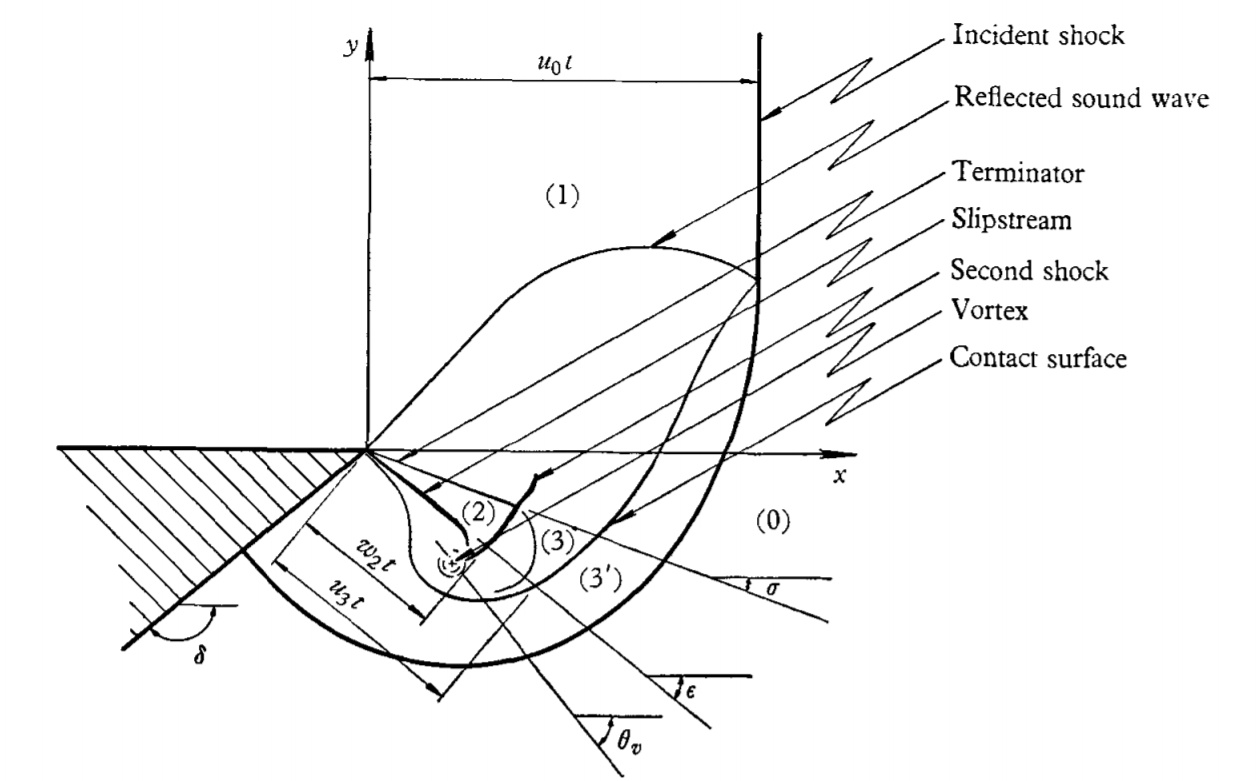
\includegraphics[scale=0.7]{fig0.PNG}
\caption{Features of the diffraction pattern \cite{skews1967}}
\label{fig:0}
\end{figure}
In the next stage, a vortex ring is generated by the roll-up of the shear layer due to Kelvin-Helmholtz type instabilities along the slipstream at the nozzle lip \cite{elder1952,dora2014}. Kelvin-Helmholtz instabilities exist within the shock as a result of external perturbations, such as inhomogeneities in the flow, producing oscillations in the vortex sheet separating fluids with different flow characteristics. This structure propagates down the jet axis, and is simultaneously accompanied by the translation of a curved barrel shock formed initially at the nozzle lip. This instigates the formation of a curved Mach disk for a ratio of the nozzle exit to free-stream pressure exceeding $2.06$ \cite{matsuda1987}. A triple point occurs between the leading edge of the barrel shock, the second shock, and the Mach disk. Given a sufficiently strong jet, a slip surface is generated downstream of the triple point. The first shock cell is formed in the third stage of jet evolution, this is marked by the pinch-off phenomenon of the vortex ring and signals the
start of the trailing jet phase \cite{gharib1998}. Separation of the vortex ring from the flow structure is driven by Kelvin-Helmholtz instabilities from the shear layer of the trailing jet \cite{zhao2000}. The final stage of the supersonic jet is defined by the point at which the transient jet and vortex are no longer joined, and the trailing jet forms. This is accompanied by the formation of a quasi-steady shock cell in self-sustained oscillation, radiating strong pressure waves. These four stages of jet evolution are illustrated in Figure \ref{fig:2}.
\begin{figure}[h] 
	\centering
	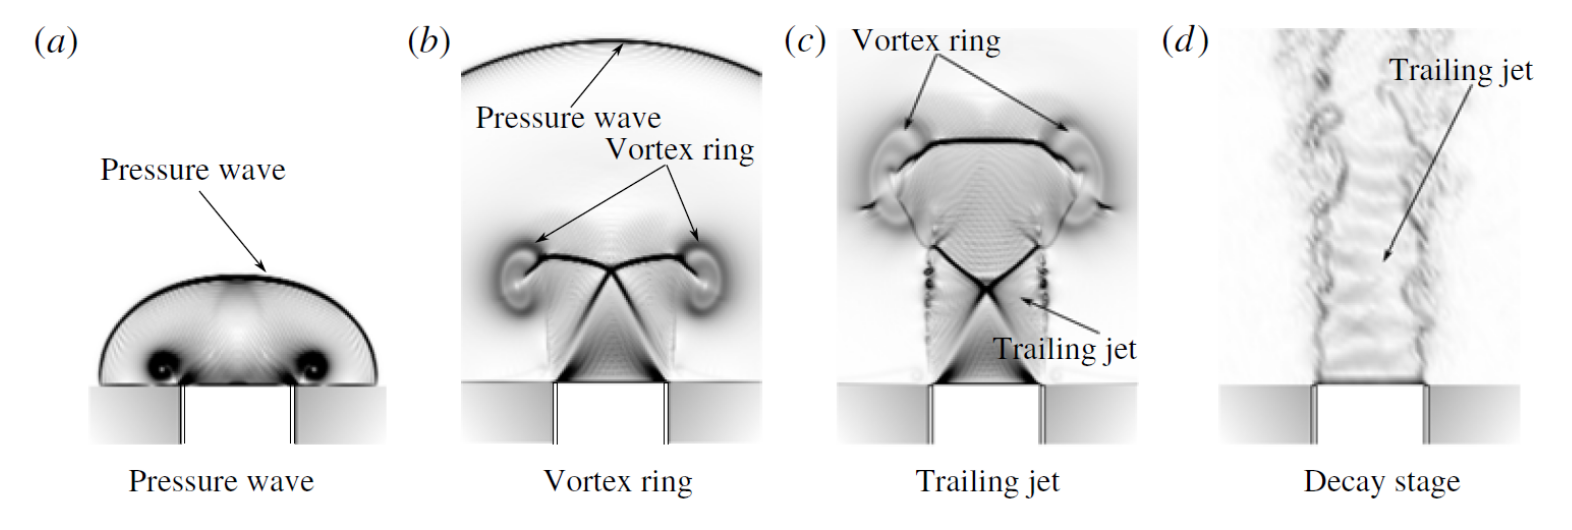
\includegraphics[scale=0.28]{fig2.png} 
	\caption{Evolution of the transient supersonic jet. (a) Diffracting shock/Pressure
		wave. (b) Axial translation of the vortex rings, formation of the curved shock and an unsteady Mach disk. (c) Formation of the trailing supersonic jet. (d) Decay of the trailing jet and the end of the transient jet
		process. \cite{fernández2017}}
	\label{fig:2}
\end{figure}

Investigation into the high pressure plenum chamber required for PDEs currently has not been undertaken although, the flow dynamics is considered similar to impingement of the transient supersonic jet on a flat plate of variable angle. The physical process is characterised initially by the reflection of the incident shock wave on the plate. This shock wave is reflected from the plate and impinges on the approaching vortex ring. The central section of the reflected shock wave is captured by the embedded rearward-facing shock at the centre of the vortex ring, and is intensified by the opposing high-speed flow. Simultaneously, the outer section of the shock wave is diffracted by the vortex core. This process results in the formation of a toroidal shock wave which focuses in the trailing jet along the longitudinal axis of flow. The next stage of fluid dynamics involves the impingement of the propagating vortex ring. Initially, as the vortex ring approaches the wall, its propagation velocity decreases and diameter increases due to the adverse pressure gradient present \cite{szumowski2000}. After impingement, the vortical flow undergoes rapid radial expansion developing a boundary layer on the surface, which slows down the flow and increases the pressure distribution over the plate. After a given duration, dependent on the initial incident Mach number, the boundary layer separates from the plate, and the flow rolls up generating a series of secondary vortices. Furthermore, the thin shear layer present between the jet flow and the exterior fluid rolls up due to Kelvin-Helmholtz instabilities. This produces small secondary vortex rings that interact with each other in propagation towards the plate \cite{minota1997}. Cumulative interactions between the primary and secondary wall vortex rings result in near standing lift off of the pair. The secondary ring subsequently merges with the primary ring, and weakened newly formed vortex ring continues to translate down the plate. Stages of impingement are illustrated in Figure \ref{fig:4} below.

\begin{figure}[h] 
	\centering
	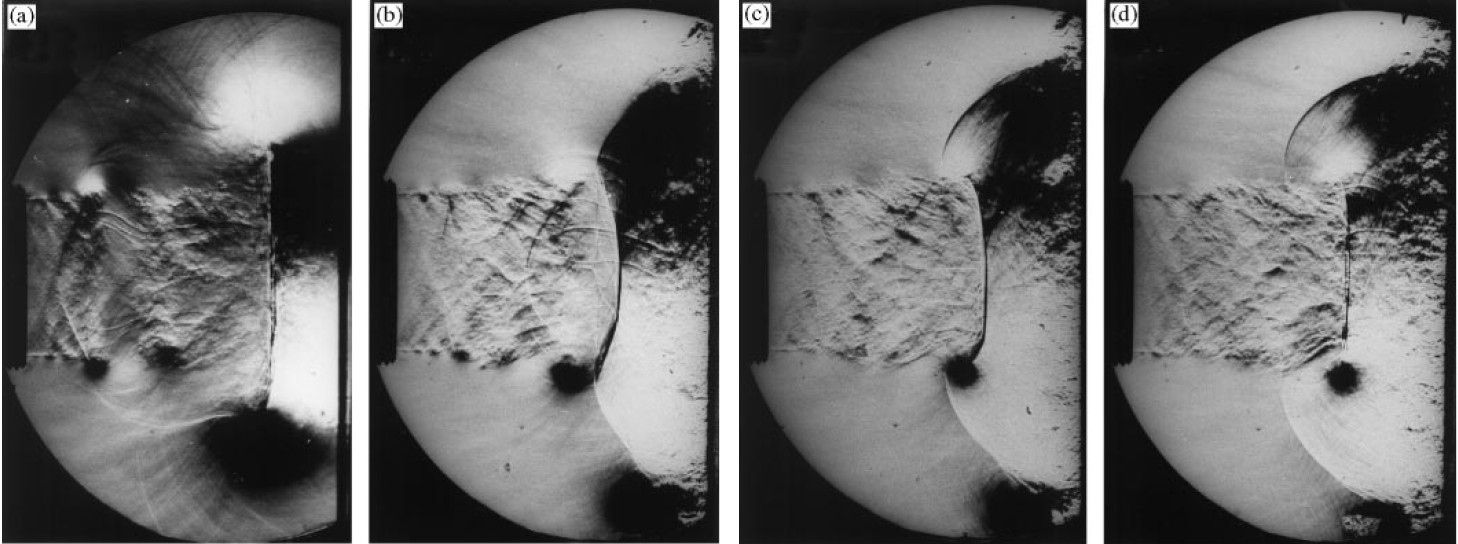
\includegraphics[scale=0.9]{fig4.PNG} 
	\caption{Evolution of jet impingement. (a) Impingement of vortex ring. (b) Vortex ring translates down the plate. (c) Secondary vortex formation. (d) Lift-off of votex rings and dissapation. \cite{szumowski2000}}
	\label{fig:4}
\end{figure}
For a plate of variable angle, the lower core of the vortex ring impinges initially, and generates an asymmetric set of secondary vortices. These new flow structures orbit around the main vortex, creating a temporarily thicker boundary layer at the lower end of the flow field. Again after a period of time, dependent on the incident Mach number, he boundary layer separates from the plate. This results in the vortex ring pivoting on the lower core, undergoing negligible deformation, towards the surface plate. The upper core then impinges on the plate and the upper wall vortex is generated. This new structure begins to expand radially increasing in thickness due to the remaining jet flow. While simultaneously, the lower wall vortex propagates around the outer limits of the main vortex, stops expanding, and dissipates into a  thin structure. The impinging jet continues to feed into the upper section of the flow field, generating  wall vortices with a thicker upper core. For lower angles of plate alignment, the flow field shows an increase in overall velocity, and visible curvature of the vortex ring structure during impingement. The toroidal shock wave that forms as a result of impingement propagates perpendicularly with respect to the surface \cite{mariani2013}.  

The far-field noise developed by the shock wave-vortex interaction can be decomposed into three components, the sound field due to the formation and evolution of the vortex ring, the reflection shock and vortex ring interaction noise production, and the noise due to impingement of the ring on the plate. The plate-votex ring impingement noise is produced by fluctuating pressure due to the deformation and stretching of the vortex ring, formation and growth of a secondary wall vortex ring, and lifting-off of the primary-secondary vortex ring pair \cite{murugan2010}.

\newpage
\section{Experimental Methods \& Analysis Techniques}

\newpage
\section{Results \& Analysis}

\newpage
\section{Discussion}

\newpage
\section{Conclusions and Recommendations}

\newpage
\section{Preliminary Results}

\subsection{Nozzle Design}

One of the first tasks completed for this project was the design and manufacture of three distinct nozzles. A convergent, divergent, and convergent-divergent nozzle was designed using CAD and manufactured by the Engineering department Mechanical Workshop. All three nozzle designs adopt geometry ratios implemented in the nozzles designed by Technical University of Berlin (TUB). Furthermore, a $60^\circ$ exterior nozzle angle and a $0.5mm$ nozzle lip was implemented in these three designs, preventing reflected flow and acoustic feedback loop interference. The three drawings for each nozzle are supplied in Appendix \ref{app:drawings}, and the manufactured parts are shown in Appendix \ref{app:manufactured}.

\subsection{Impingement Plate Design}
The impingement plate, as shown in appendix \ref{app:drawings}, is constructed such that it is $90^{\circ}$ to the direction of the flow. It mounted on rails which fix to the shock tube rig, this construction can be adjusted to 1 and 4 inner diameters. The plate is fixed to the rails such that it can be removed and replaced with another plate of alternate geometry for future research. During the evolution of a transient supersonic jet, the vortex is fully formed at approximately 3 inner diameters, from the exit for a conventional, no nozzle, shock tube \cite{mariani2013a}. As a result, an impingement plate distance is chosen below and above this limit, at 1 and 4 inner diameters, respectively. Moreover, the plate diameter is designed such that it appears infinite to the flow, to maintain consistency with the literature.

\subsection{Literature Comparison}
Initially, it is necessary to explore the literature and develop an understanding of the current comprehension of the flow characteristics governing supersonic transient jet impingement, and previous experimental test configurations. Section \ref{sec:background} undertakes an extensive review of previous literature, exploring the fluid dynamics and practical applications of supersonic impinging jets. Table \ref{tab1} details a summary for the research undertaken in previous literature, it's important to note all previous literature sources implement a plate diameter such that it can be considered infinite to the flow. Additionally, imaging results from the literature summarised in Table 1 is subsequently shown in appendix \ref{app:litresults}.

\begin{table}[h]
	\centering
	\caption{Literature Summary}
	\label{tab1}
	\resizebox{\textwidth}{!}{ 
		\begin{tabular}{@{}llllll@{}}
			\toprule
			Paper                                                                                                                           & \begin{tabular}[c]{@{}l@{}}Main\\ Research\\ Focus\end{tabular}                                                          & \begin{tabular}[c]{@{}l@{}}Imaging\\ Technique\end{tabular}                                            & \begin{tabular}[c]{@{}l@{}}Inner Shock\\ Tube\\ Diameter\end{tabular} & \begin{tabular}[c]{@{}l@{}}Incident\\ Mach\\ Number\end{tabular} & \begin{tabular}[c]{@{}l@{}}Impingement\\ Plate Distance\\ (inner diameter)\end{tabular}   \\ \midrule
			\multicolumn{1}{|l|}{\cite{minota1997}}                                                                                              & \multicolumn{1}{l|}{\begin{tabular}[c]{@{}l@{}}Shock-vortex \\ interaction in \\ the flow field\end{tabular}}            & \multicolumn{1}{l|}{Shadowgraph}                                                                       & \multicolumn{1}{l|}{40mm}                                             & \multicolumn{1}{l|}{1.35}                                        & \multicolumn{1}{l|}{0.4di}                                                                \\ \midrule
			\multicolumn{1}{|l|}{\cite{szumowski2000}}                                                                                              & \multicolumn{1}{l|}{\begin{tabular}[c]{@{}l@{}}Sound generation \\ upon impingement\end{tabular}}                        & \multicolumn{1}{l|}{schlieren}                                                                         & \multicolumn{1}{l|}{65mm}                                             & \multicolumn{1}{l|}{1.14}                                        & \multicolumn{1}{l|}{2di}                                                                  \\ \midrule
			\multicolumn{1}{|l|}{\cite{murugan2010}}                                                                                              & \multicolumn{1}{l|}{\begin{tabular}[c]{@{}l@{}}Noise due to shock-\\ vortex interaction \\ and impingement\end{tabular}} & \multicolumn{1}{l|}{\begin{tabular}[c]{@{}l@{}}High-speed\\ smoke flow\\ visualisations.\end{tabular}} & \multicolumn{1}{l|}{64mm}                                             & \multicolumn{1}{l|}{1.31 - 1.55}                                 & \multicolumn{1}{l|}{4.7di}                                                                \\ \midrule
			\multicolumn{1}{|l|}{\cite{murugan2012}}                                                                                              & \multicolumn{1}{l|}{\begin{tabular}[c]{@{}l@{}}Vortex ring\\ impingement\end{tabular}}                                   & \multicolumn{1}{l|}{\begin{tabular}[c]{@{}l@{}}High-speed\\ smoke flow\\ visualisations.\end{tabular}} & \multicolumn{1}{l|}{64mm}                                             & \multicolumn{1}{l|}{1.31 - 1.85}                                 & \multicolumn{1}{l|}{4.7di}                                                                \\ \midrule
			\multicolumn{1}{|l|}{\cite{mariani2013a}}                                                                                              & \multicolumn{1}{l|}{\begin{tabular}[c]{@{}l@{}}Vortex ring\\ impingement\end{tabular}}                                   & \multicolumn{1}{l|}{schlieren}                                                                         & \multicolumn{1}{l|}{30mm}                                             & \multicolumn{1}{l|}{1.61}                                        & \multicolumn{1}{l|}{\begin{tabular}[c]{@{}l@{}}1.66di, \\ 3.33di, \\ 5.00di\end{tabular}} \\ \bottomrule
		\end{tabular}}
	\end{table}
	
\subsection{Saftey Documentation} 
The safety documentation is completed using Monash Universities Safety and Risk Analysis Hub (S.A.R.A.H.). This is included in Appendix \ref{app:safety}.

\section{Research Plan}

\subsection{Projected Research Stages}

The project has been divided into separate stages with individual tasks and outcomes. These stages are listed in a progression although, it is expected that most will run concurrently. Whilst only listed under Stage 1 explicitly, a constant review of literature will be conducted throughout the project.

\subsubsection*{Stage 1:}
\begin{itemize}
	\item Explore the literature to identify the position of the project.
	\item Establish the theoretical basis for various parts of the project including fundamental aerodynamics and measurements techniques.
\end{itemize}
\textbf{Outcomes:} Continually develop an understanding of the literature and expand background knowledge.

\subsubsection*{Stage 2:}
\begin{itemize}
	\item Participate in schlieren measurements of supersonic flow with PhD students.
	\item Complete necessary safety and training inductions, developing safe work instructions and undertaking risk assessments.
\end{itemize}
\textbf{Outcomes:} Proficiency in the OHS requirements of the Supersonic Jet Facility. Develop schlieren imagining skills.

\subsubsection*{Stage 3:}
\begin{itemize}
	\item Characterise nozzles and perform schlieren on transient supersonic jets.
	\item Analysis of transient supersonic jet data to produce qualitatively comparable results.
\end{itemize}
\textbf{Outcomes:} Produce data set for each of the three nozzle designs to be used for later data analysis. Provide qualitative results for comparison with the literature.

\subsubsection*{Stage 4:}
\begin{itemize}
	\item Introduce impingement plate and record data.
	\item Conduct parameter sweep and identify a parameter space.
\end{itemize}
\textbf{Outcomes:} Develop impingement data set to be used for data analysis.

\subsubsection*{Stage 5:}                                 
\begin{itemize}
	\item Identification of trends within the data for both transient supersonic flow and jet impingement.
\end{itemize}
\textbf{Outcomes:} Comparison of transient supersonic jet impingement with the literature. Improved understanding of the interaction phenomenon.

\subsection{Experimental Methodology}
To further understand the impingement of transient supersonic jets, the Laboratory for Turbulence Research in Aerospace and Combustion (LTRAC) Supersonic Jet Facility will be utilised. A schematic of the facility is shown in Appendix \ref{app:facility}. The facility utilises compressed air delivered by the Monash University compressed air supply system. To produce a canonical transient supersonic jet, a shock tube model is adopted \cite{bradley1962}. A typical shock tube consists of a high pressure section (driver section) and a low pressure section (driven section) separated by a diaphragm. Air enters the driver section until a desired pressure is reached, the diaphragm is then ruptured via an actuated pin or knife that punctures the diaphragm. Following the rupture, compression waves are fired down the driven section by the high pressure gas in the driver. As these compression waves travel down the tube, they coalesce and form a shock wave that propagates into the test section, diffracts, and produces a transient supersonic jet. 
\\\\
In this experiment, the supersonic transient jet will be studied with varied nozzle designs including a convergent, divergent and convergent-divergent configuration. Furthermore, transient flow impingement will be tested via a flat plate set at $90^{\circ}$ to the flow. This impinging plate is set exactly at an angle of $90^{\circ}$ to the flow by a connection to an already manufactured $90^{\circ}$ component of the shock facility, and the plate itself having manufacture specifications of exactly $90^{\circ}$. The three nozzle designs and impingement plate will be integrated into the existing LTRAC Supersonic Jet Facility. For further details on the design and manufacture of the nozzles, or the impingement plate, please see Appendix \ref{app:drawings}. In order to study the features of the flow, schlieren imaging techniques will be implemented in the test facility.

\subsection{Schlieren Imaging}
Schlieren imaging is a visualization technique that utilises the refraction of light to produce focused optical images of transparent media. Point source light is collimated and passed through a test region containing a transparent media with inhomogeneities.  Light entering the test region will refract at varied degrees according to an inhomogeneous density distribution present. The light is then refocused and a knife-edge is used to partially block a fraction of incident light from the screen or camera. 

This experiment will implement the most common schlieren technique used, a Z-type schlieren apparatus (illustrated in Figure \ref{fig:3}) with the Shimadzu HPV-1 camera. The Shimadzu has a resolution of 312 x 260 pixels and a frame rate of up to 1 million fps. Table \ref{tab2} details certain schlieren configuration specifications, it's important to note this is only a guide based on equations derived in \cite{settles2012}, and implementing these configurations in the lab maybe differ slightly.

It's important to note, schlieren imaging has a number of limitations. Firstly, schlieren images are constructed using density gradients within the test region. The gradients are integrated over the optical path and images are therefore developed as two-dimensional projections of an original three-dimensional fluid flow. This introduces possible incorrect projects of three-dimensional features. Furthermore, the technique is line-of-sight dependent, as the light must be collimated and refocused in order to produce an image. This restricts the layout of test section and sets requirements on the amount of space required for the apparatus. 

\begin{figure}[H] 
	\centering
	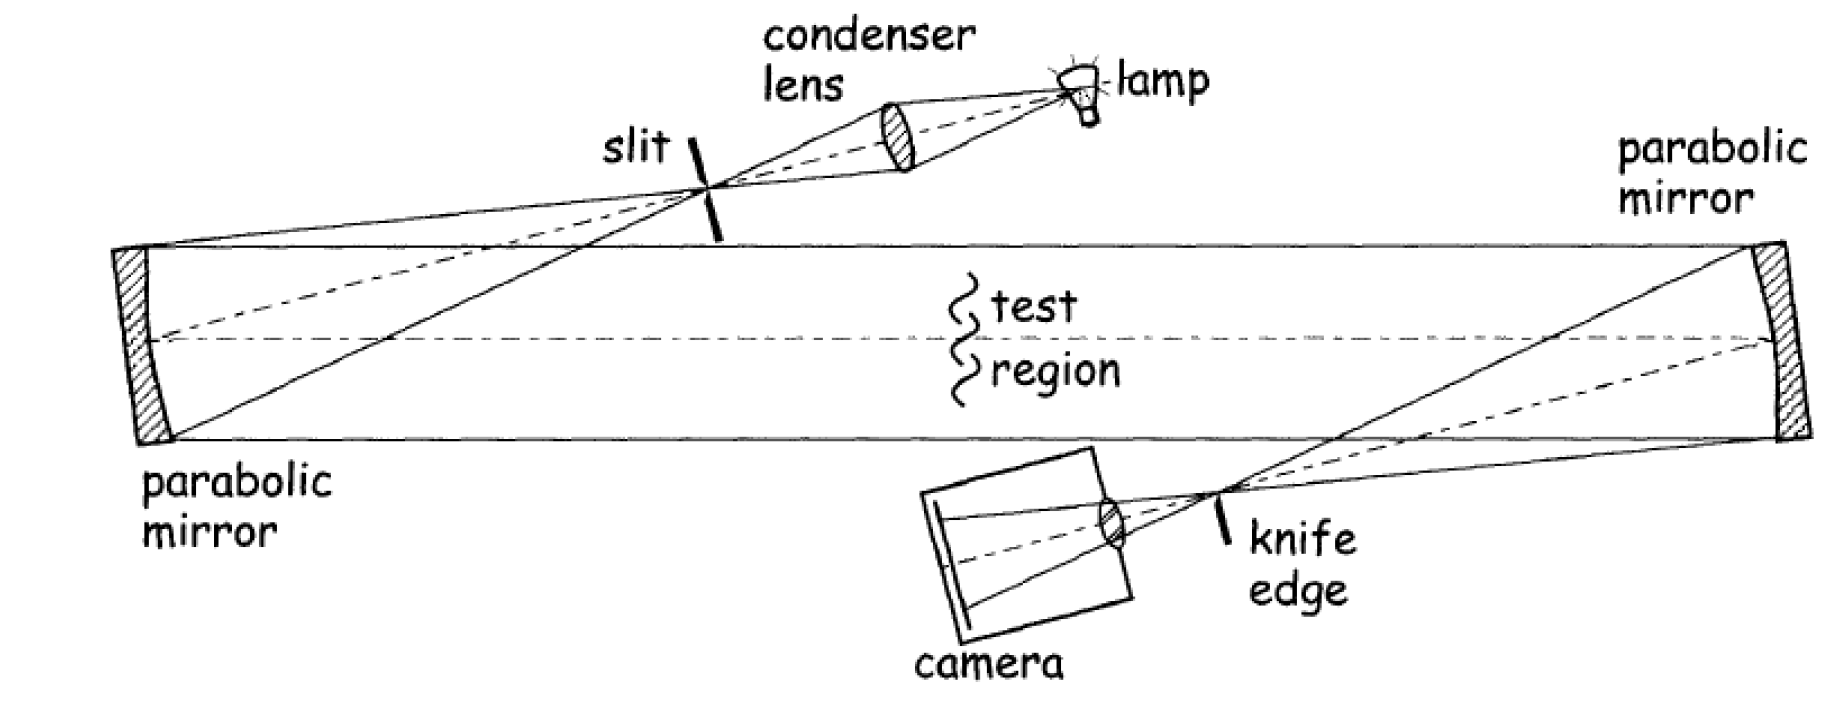
\includegraphics[scale=0.7]{fig3.PNG} 
	\caption{Diagram of the second field mirror and analyzer section of a z-type schlieren
		system showing notation regarding magnification and the focusing lens \cite{settles2012}.}
	\label{fig:3}
\end{figure}

\begin{table}[h]
	\centering
	\caption{Schlieren Configuration Specifications}
	\label{tab2}
	\begin{tabular}{@{}lllll@{}}
		\toprule
		optical view mm & g distance & lens FL  & e distance \\ \midrule
		3.12            & 50.00      & 0.00     & 0.00       \\
		5.55            & 61.11      & 111.11   & 111.07     \\
		7.97            & 72.22      & 222.22   & 221.96     \\
		10.40           & 83.33      & 333.33   & 332.56     \\
		12.83           & 94.44      & 444.44   & 442.75     \\
		15.25           & 105.56     & 555.56   & 552.40     \\
		17.68           & 116.67     & 666.67   & 661.41     \\
		20.11           & 127.78     & 777.78   & 769.67     \\
		22.53           & 138.89     & 888.89   & 877.05     \\
		24.96           & 150.00     & 1,000.00 & 983.44     \\ \bottomrule
	\end{tabular}
\end{table}

\subsection{Flow Field}
This experiment aims to explore 3 characteristic flow regimes including; subsonic impingement with an incident Mach number of 1.2 and a pressure ratio of 1.805, transition regime flow with an incident Mach number of 1.7 and a pressure ratio of 5.57, and supersonic post shock flow with an incident Mach number of 2.3 and a pressure ratio of 15.85 (In these cases, incident Mach number refers to the Mach number of the initial shock wave formed upon exit of the transient flow from the nozzle). It's important to note these Mach values are only theoretical and the relation shown in Figure \ref{fig:1} are for the ideal case. Practical results will vary as there numerous avenues for energy dissipation in the test system. Additionally, a reference for the relation between exit Mach number and pressure ratio is shown. This is included to illustrate the advantages of implementing helium as the driving gas in the shock tube. Helium gas delivers a much more significant incident Mach for an insignificant increase in pressure ratio when in comparison to air. The derivation of this relation is shown in the appendix \ref{app:shock}. 

\begin{figure}[H] 
	\centering
	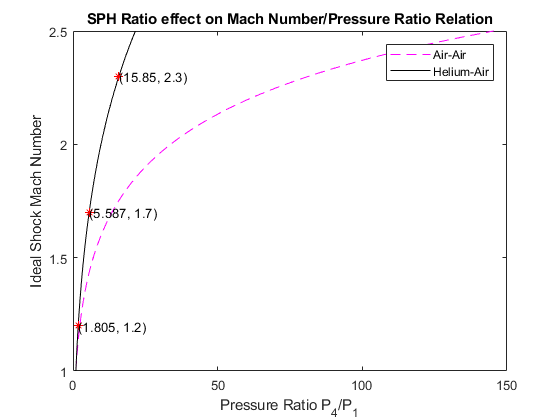
\includegraphics[scale=0.9]{fig1.png} 
	\caption{Specific Heat Capacity Ratio effect on Mach Number/Pressure Ratio.}
	\label{fig:1}
\end{figure}

\subsection{Results Analysis and Discussion}
The analysis of the schlieren image results and following flow field analysis is integral to any meaningful outcome of research. The motivations for this research are, as summarised:  

\begin{itemize}
	\item Nozzle geometry effects on the shock-vortex interaction and jet impingement
	\item Counter rotating vortex rings (CRVR) interactions
	\item Acoustic feedback characteristics
	\item Mach number variations on all the above
\end{itemize}
Specifically, the analysis of the flow field will involve writing a code that can analyse and extract the position of the shock waves (most likely based upon an edge detection method). From this we can quantify; the position of the Mach disk from nozzle exit (for different geometries and plate heights), and then use this to quantify the effect of variable nozzle geometries, incident Mach numbers and plate heights. Additionally, a visual analysis will be undertaken to identify and compare features of instantaneous images for different nozzle geometries, to further understand; Mach disk formation, evidence of counter rotating vortices, and plate effects.
\newpage
\footnotesize
\begin{thebibliography}{99}
\addcontentsline{toc}{section}{References}
	\bibitem [Bradley (1962)]{bradley1962}
	John N. Bradley. (1962). \textit{Shock waves in chemistry and physics}. Methuen.
	\bibitem [Cantwell (2017)]{cantwell2017}
	Cantwell, B. (2017).
	Fundamentals of Compressible Flow. \textit{Standford Aeronautics and Astronautics}, Ch13.7
	\bibitem [Dean et al.(2005)]{dean2005}
	Dean, A. J., Rasheed, A., Tangirala, V., \& Pinard, P. F. (2005, January). Operation and noise transmission of an axial turbine driven by a pulse detonation combustor. In \textit{ASME Turbo Expo 2005: Power for Land, Sea, and Air} (pp. 1275-1284). American Society of Mechanical Engineers.
	\bibitem [Dora et al.(2014)]{dora2014}
	Dora, C. L., Murugan, T., De, S., \& Das, D. (2014). Role of slipstream instability in formation of counter-rotating vortex rings ahead of a compressible vortex ring. \textit{Journal of Fluid Mechanics}, 753, 29-48.
	\bibitem [Eidelman et al.(1991)]{eidelman1991}
	Eidelman, S., Grossmann, W., \& Lottati, I. (1991). Review of propulsion applications and numerical simulations of the pulsed detonation engine concept. \textit{Journal of Propulsion and Power}, 7(6), 857-865.
	\bibitem [Elder \& De Haas (1952)]{elder1952}
	Elder Jr, F. K., \& De Haas, N. (1952). Experimental study of the formation of a vortex ring at the open end of a cylindrical shock tube. \textit{Journal of Applied Physics}, 23(10), 1065-1069.
	\bibitem [Fernández \& Sesterhenn (2017)]{fernández2017}
	Fernández, J. J. P., \& Sesterhenn, J. (2017). Compressible starting jet: pinch-off and vortex ring–trailing jet interaction. \textit{Journal of Fluid Mechanics}, 817, 560-589.
	\bibitem [G\"ulen (2013)]{gulen2013}
	G\"ulen, S. C. (2013). Constant volume combustion: The ultimate gas turbine cycle. \textit{Gas Turbine World}, 43(6), 20-27.
	\bibitem [Gharib et al.(1998)]{gharib1998}
	Gharib, M., Rambod, E., \& Shariff, K. (1998). A universal time scale for vortex ring formation. \textit{Journal of Fluid Mechanics}, 360, 121-140.
	\bibitem [Ishii (1999)]{ishii1999}
	Ishii, R., Fujimoto, H., Hatta, N., \& Umeda, Y. (1999). Experimental and numerical analysis of circular pulse jets. \textit{Journal of Fluid Mechanics}, 392, 129-153.
	\bibitem [Kailasanath (2009)]{kailasanath2009}
	Kailasanath, K. (2009, January). Research on pulse detonation combustion systems: a status report. In \textit{47th AIAA Aerospace Sciences Meeting Including The New Horizons Forum and Aerospace Exposition} (p. 631).
	\bibitem[Kleine et al.(1995)]{kleine1995}
	Kleine, H., Ritzerfeld, E., \& Grönig, H. (1995). Shock wave diffraction—new aspects of an old problem. \textit{In Shock Waves@ Marseille IV} (pp. 117-122). Springer, Berlin, Heidelberg.
	\bibitem[Mariani et al.(2013)]{mariani2013a}
	Mariani, R., Kontis, K., \& Gongora-Orozco, N. (2013). Head on collisions of compressible vortex rings on a smooth solid surface. \textit{Shock Waves}, 23(4), 381-398.
	\bibitem [Mariani et al.(2013)]{mariani2013}
	Mariani, R., Quinn, M. K., Kontis, K., \& Marraffa, L. (2013). Shock-free compressible vortex rings impinging on a stationary surface: Effects of surface angle variation. \textit{Experimental Thermal and Fluid Science}, 47, 126-142.
	\bibitem [Matsuda et al.(1987)]{matsuda1987}
	MATSUDA, T., UMEDA, Y., ISHII, R., \& SAWADA, K. (1987). Numerical and experimental studies on choked underexpanded jets. In \textit{19th AIAA, Fluid Dynamics, Plasma Dynamics, and Lasers Conference} (p. 1378).
	\bibitem[Minota et al.(1997)]{minota1997}
	Minota, T., Nishida, M., \& Lee, M. G. (1997). Shock formation by compressible vortex ring impinging on a wall. \textit{Fluid dynamics research}, 21(3), 139.
	\bibitem[Murugan \& Das (2010)]{murugan2010}
	Murugan, T., \& Das, D. (2010). Characteristics of noise produced during impingement of a compressible vortex ring on a wall. \textit{International Journal of Aeroacoustics}, 9(6), 849-858.
	\bibitem[Murugan \& Das (2012)]{murugan2012}
	Thangadurai, M., \& Das, D. (2012). Experimental study on a compressible vortex ring in collision with a wall. Journal of visualization, 15(4), 321-332.
	\bibitem [Paxon (2010)]{paxson2010} 
	D Paxson. (2010). Pressure-gain combustion for the gas turbine. \textit{In University Turbine Systems Research Workshop}. Pennsylvania State University.
	\bibitem [Radulescu \& Law (2007)]{radulescu2007}
	Radulescu, M. I., \& Law, C. K. (2007). The transient start of supersonic jets. \textit{Journal of Fluid Mechanics}, 578, 331-369.
	\bibitem[Settles (2012)]{settles2012}
	Settles, G. S. (2012). \textit{Schlieren and shadowgraph techniques: visualizing phenomena in transparent media. Springer Science \& Business Media}.
	\bibitem [Skews 1967]{skews1967}
	Skews, B. W. (1967). The perturbed region behind a diffracting shock wave. \textit{Journal of Fluid Mechanics}, 29(4), 705-719.
	\bibitem[Szumowski et al.(2000)]{szumowski2000}
	Szumowski, A., Sobieraj, G., Selerowicz, W., \& Piechna, J. (2000). Starting jet–wall interaction. \textit{Journal of sound and vibration}, 232(4), 695-702.
	\bibitem [Zhao et al.(2000)]{zhao2000}
	Zhao, W., Frankel, S. H., \& Mongeau, L. G. (2000). Effects of trailing jet instability on vortex ring formation. \textit{Physics of Fluids}, 12(3), 589-596.


\end{thebibliography}

%----------------------------------------------------------------------------------------
\normalsize
\newpage

\appendix
\addcontentsline{toc}{section}{Appendix}

\section{Shock Facility} \label{app:facility}

\begin{figure}[H] 
	\centering
	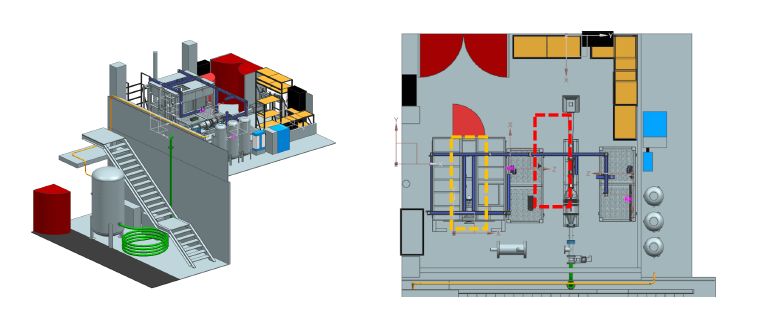
\includegraphics[width=1.05\textwidth]{fig10.PNG} 
	\caption{(Left): Isometric view of the LTRAC Shock Lab, with the shock tube facility stored under the
		shelving. (Right): Top view of the LTRAC Shock Lab, with the PIV (orange) and schlieren (red) sites
		highlighted.}
	\label{fig:10}
\end{figure}

\begin{figure}[H] 
	\centering
	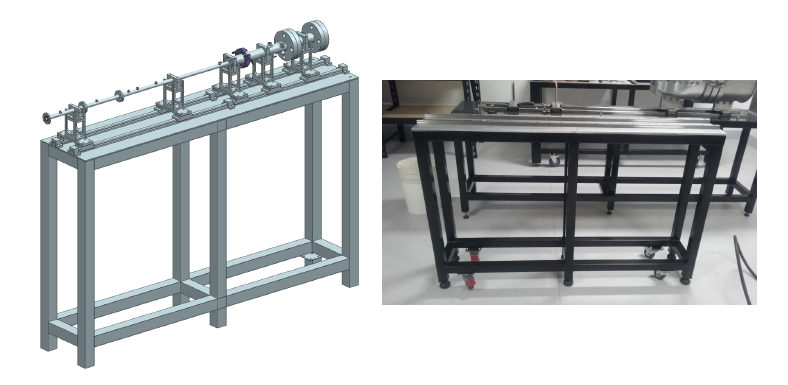
\includegraphics[width=1.05\textwidth]{fig8.PNG} 
	\caption{Isometric view of the design of the shock tube facility. (Right): Progress of the commission
		of the shock tube facility.}
	\label{fig:8}
\end{figure}

\begin{figure}[H] 
	\centering
	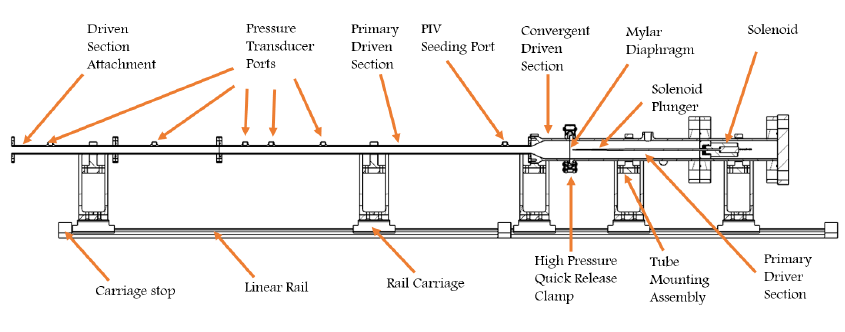
\includegraphics[width=1.05\textwidth]{fig9.PNG} 
	\caption{Schematic diagram of the shock tube facility currently under commission. Major parts of the
		system have been labelled.}
	\label{fig:9}
\end{figure}	

\section{Nozzle and Plate Design} \label{app:drawings}



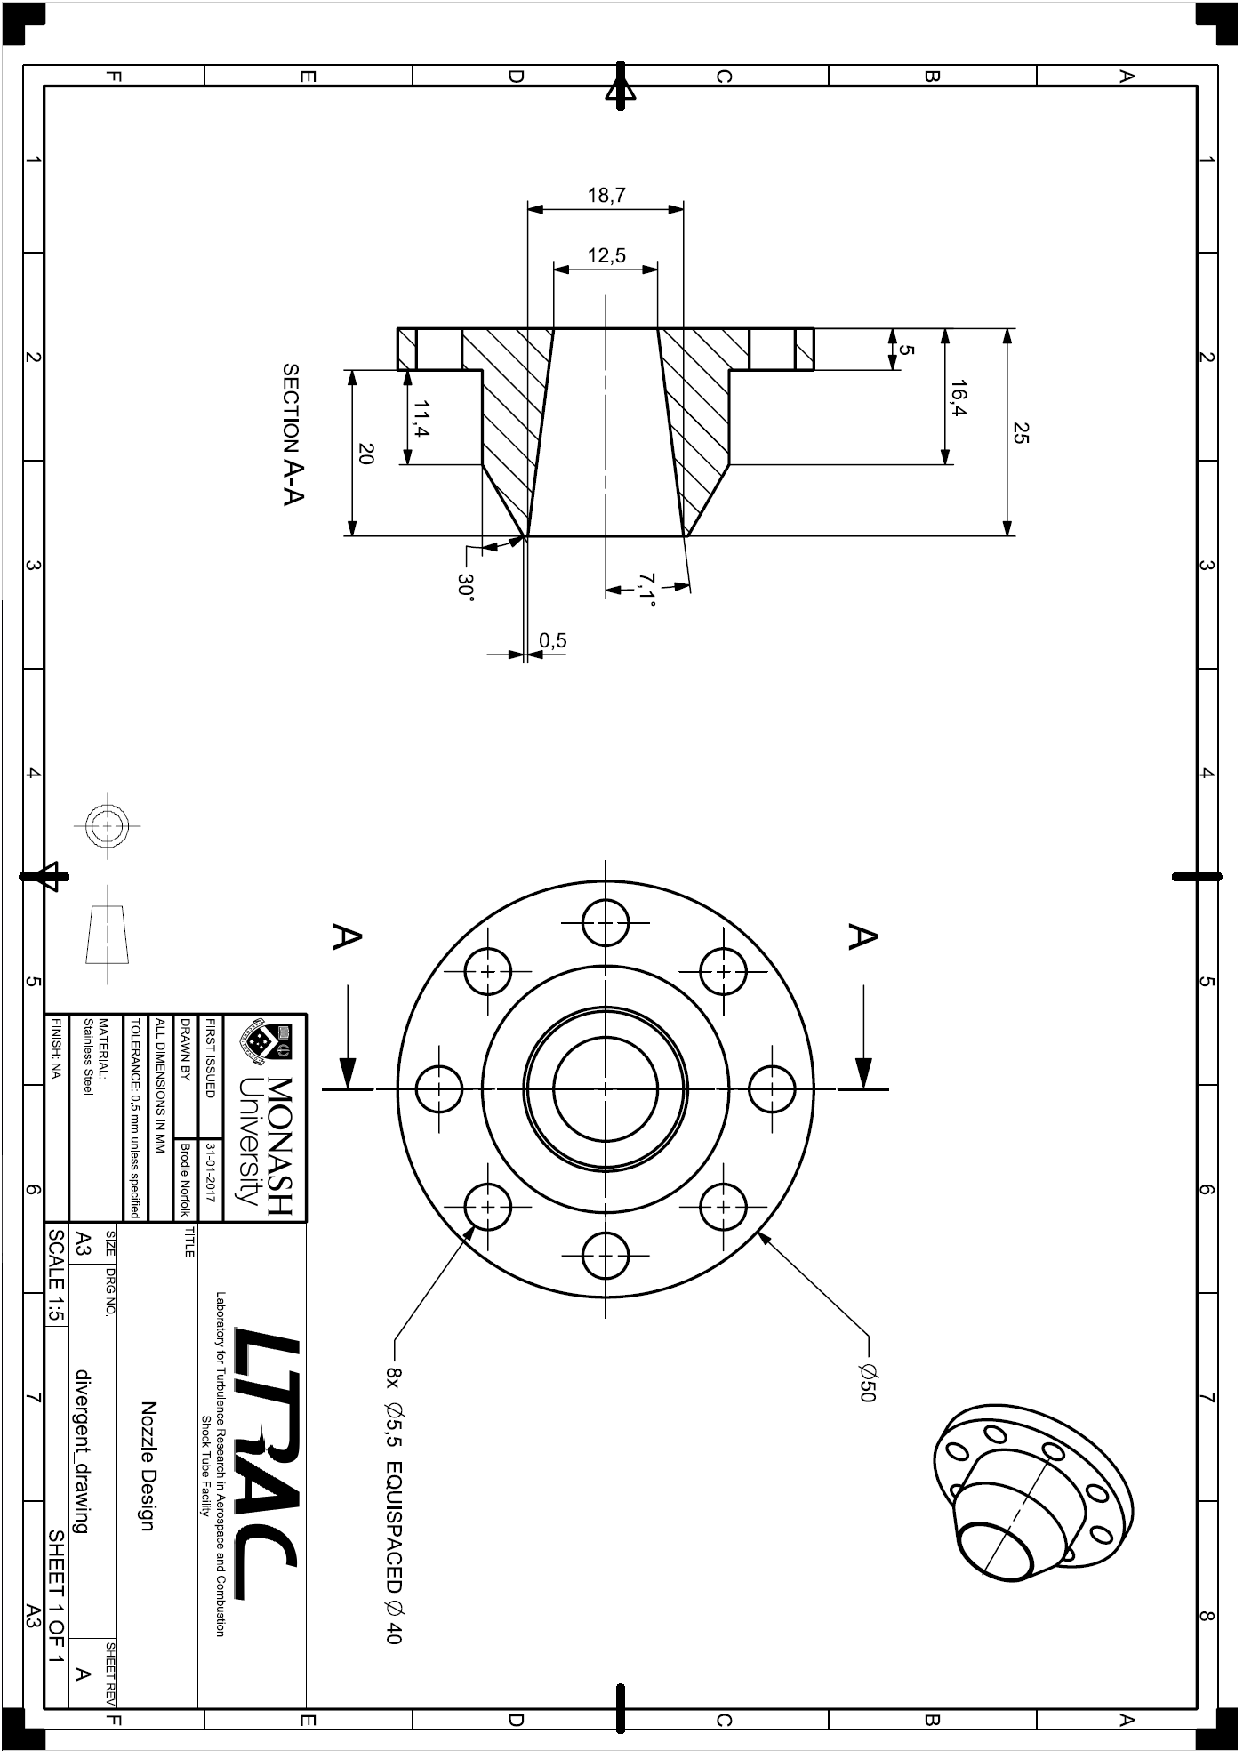
\includepdf[pages={-},angle=90,fitpaper,pagecommand={}]{fig5.pdf}

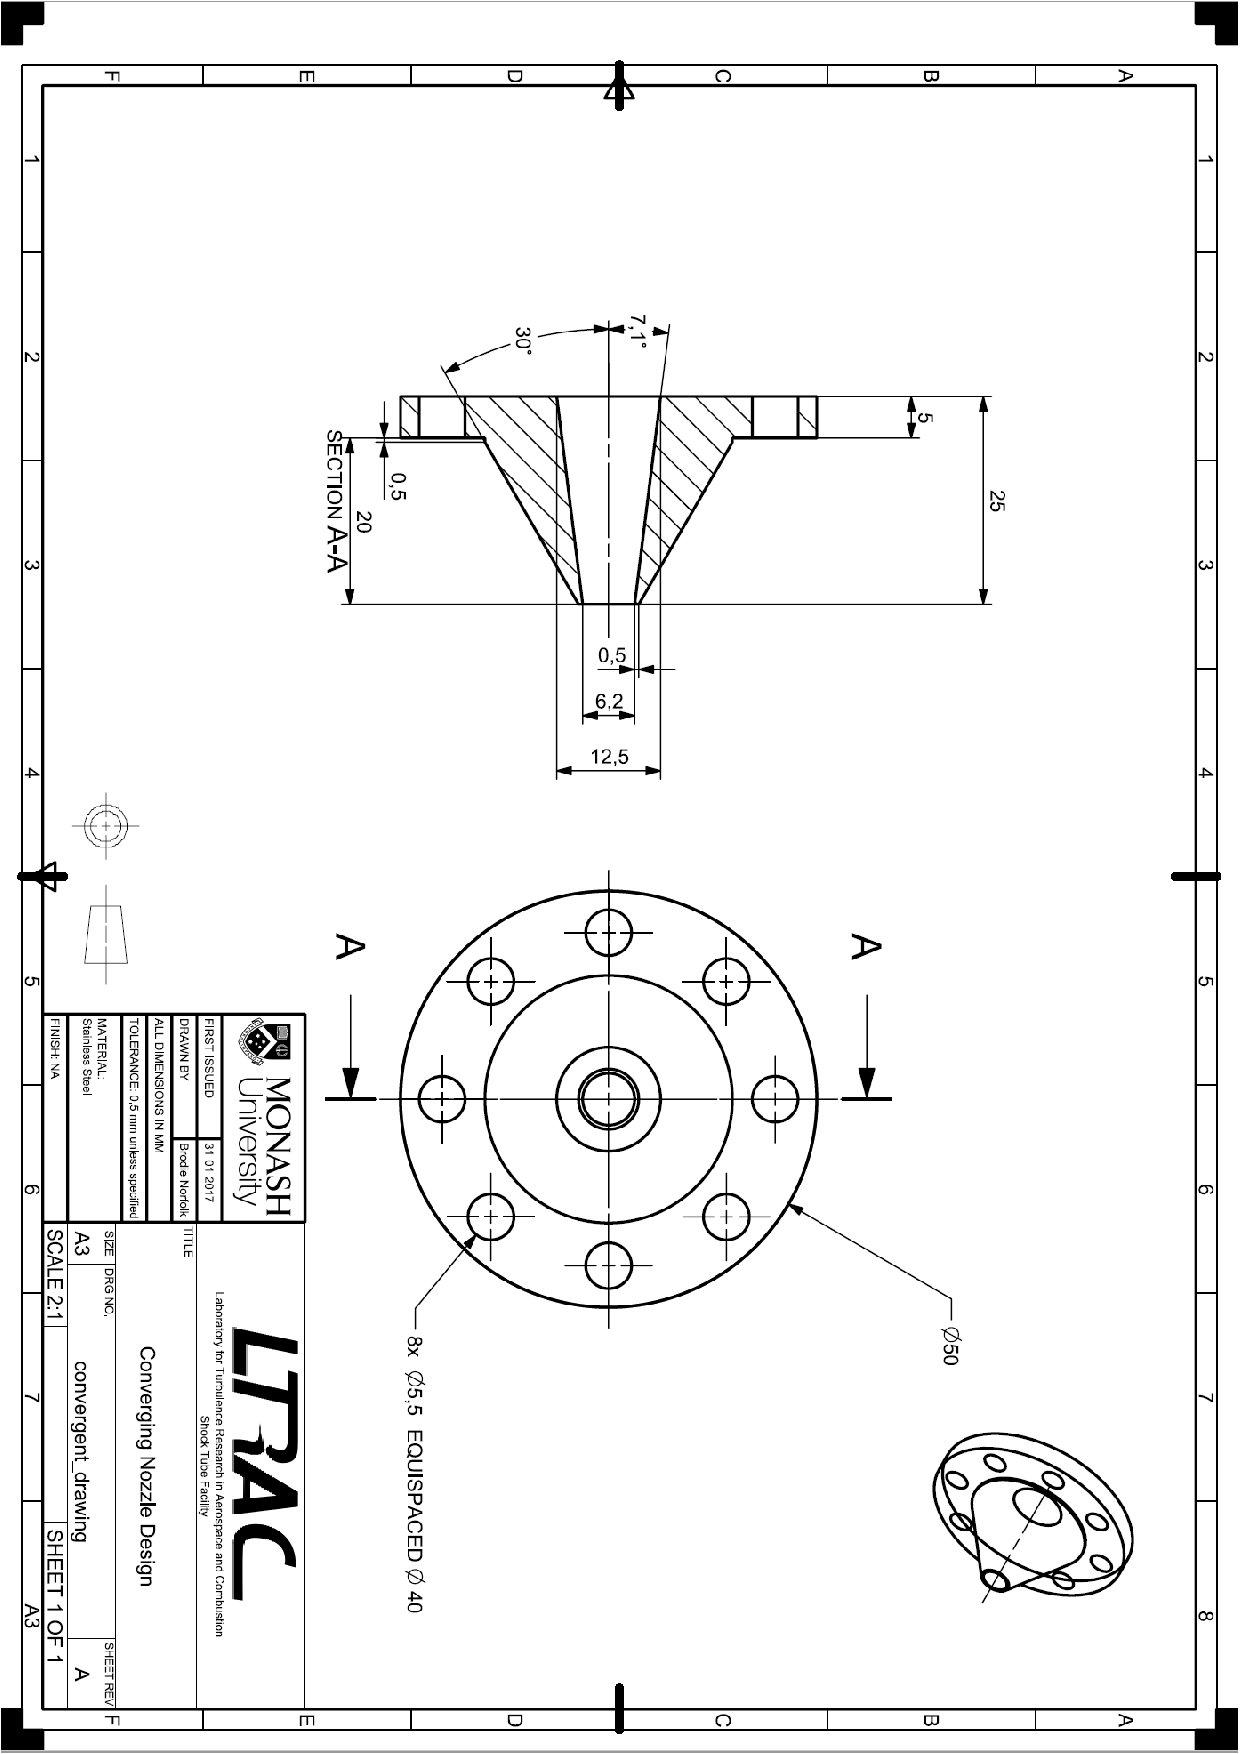
\includepdf[pages={-},angle=90,fitpaper,pagecommand={}]{fig6.pdf}

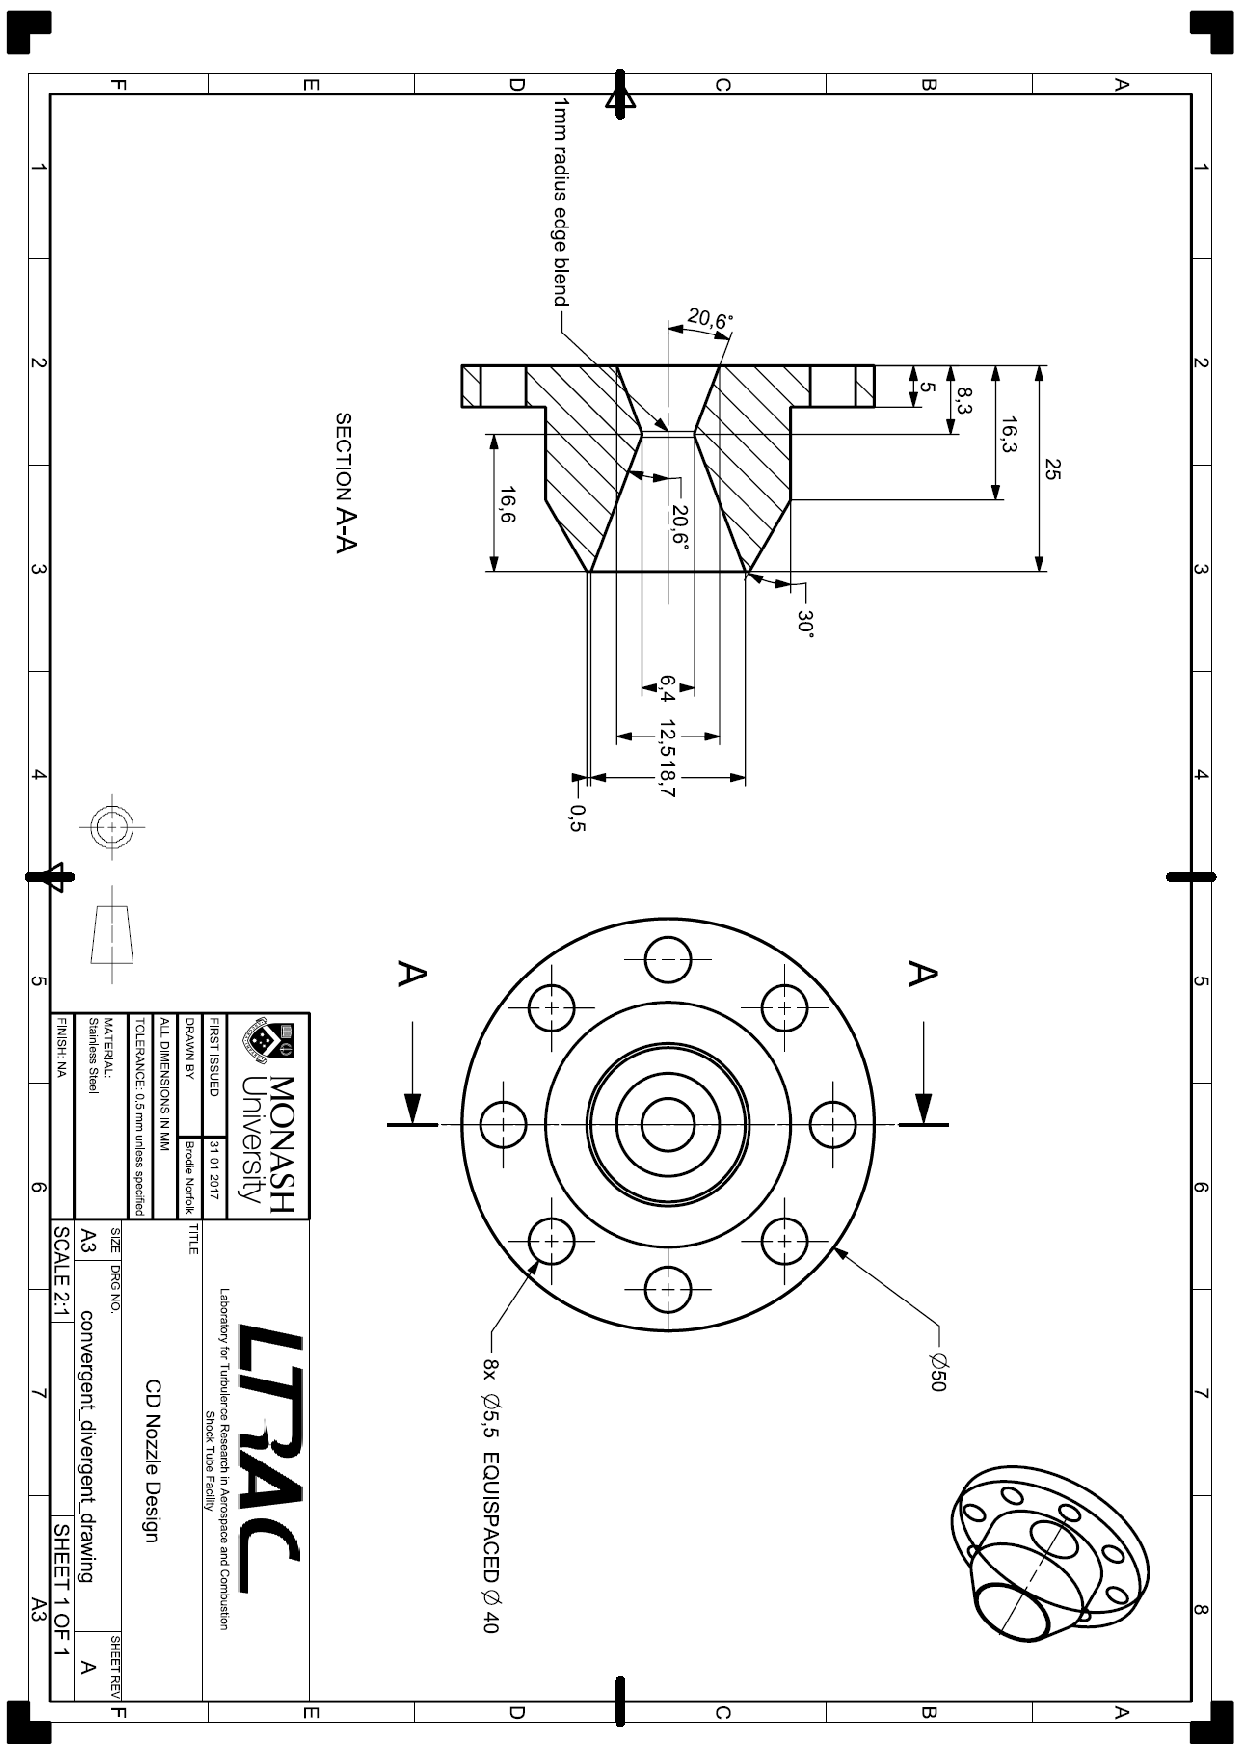
\includepdf[pages={-},angle=90,fitpaper,pagecommand={}]{fig7.pdf}
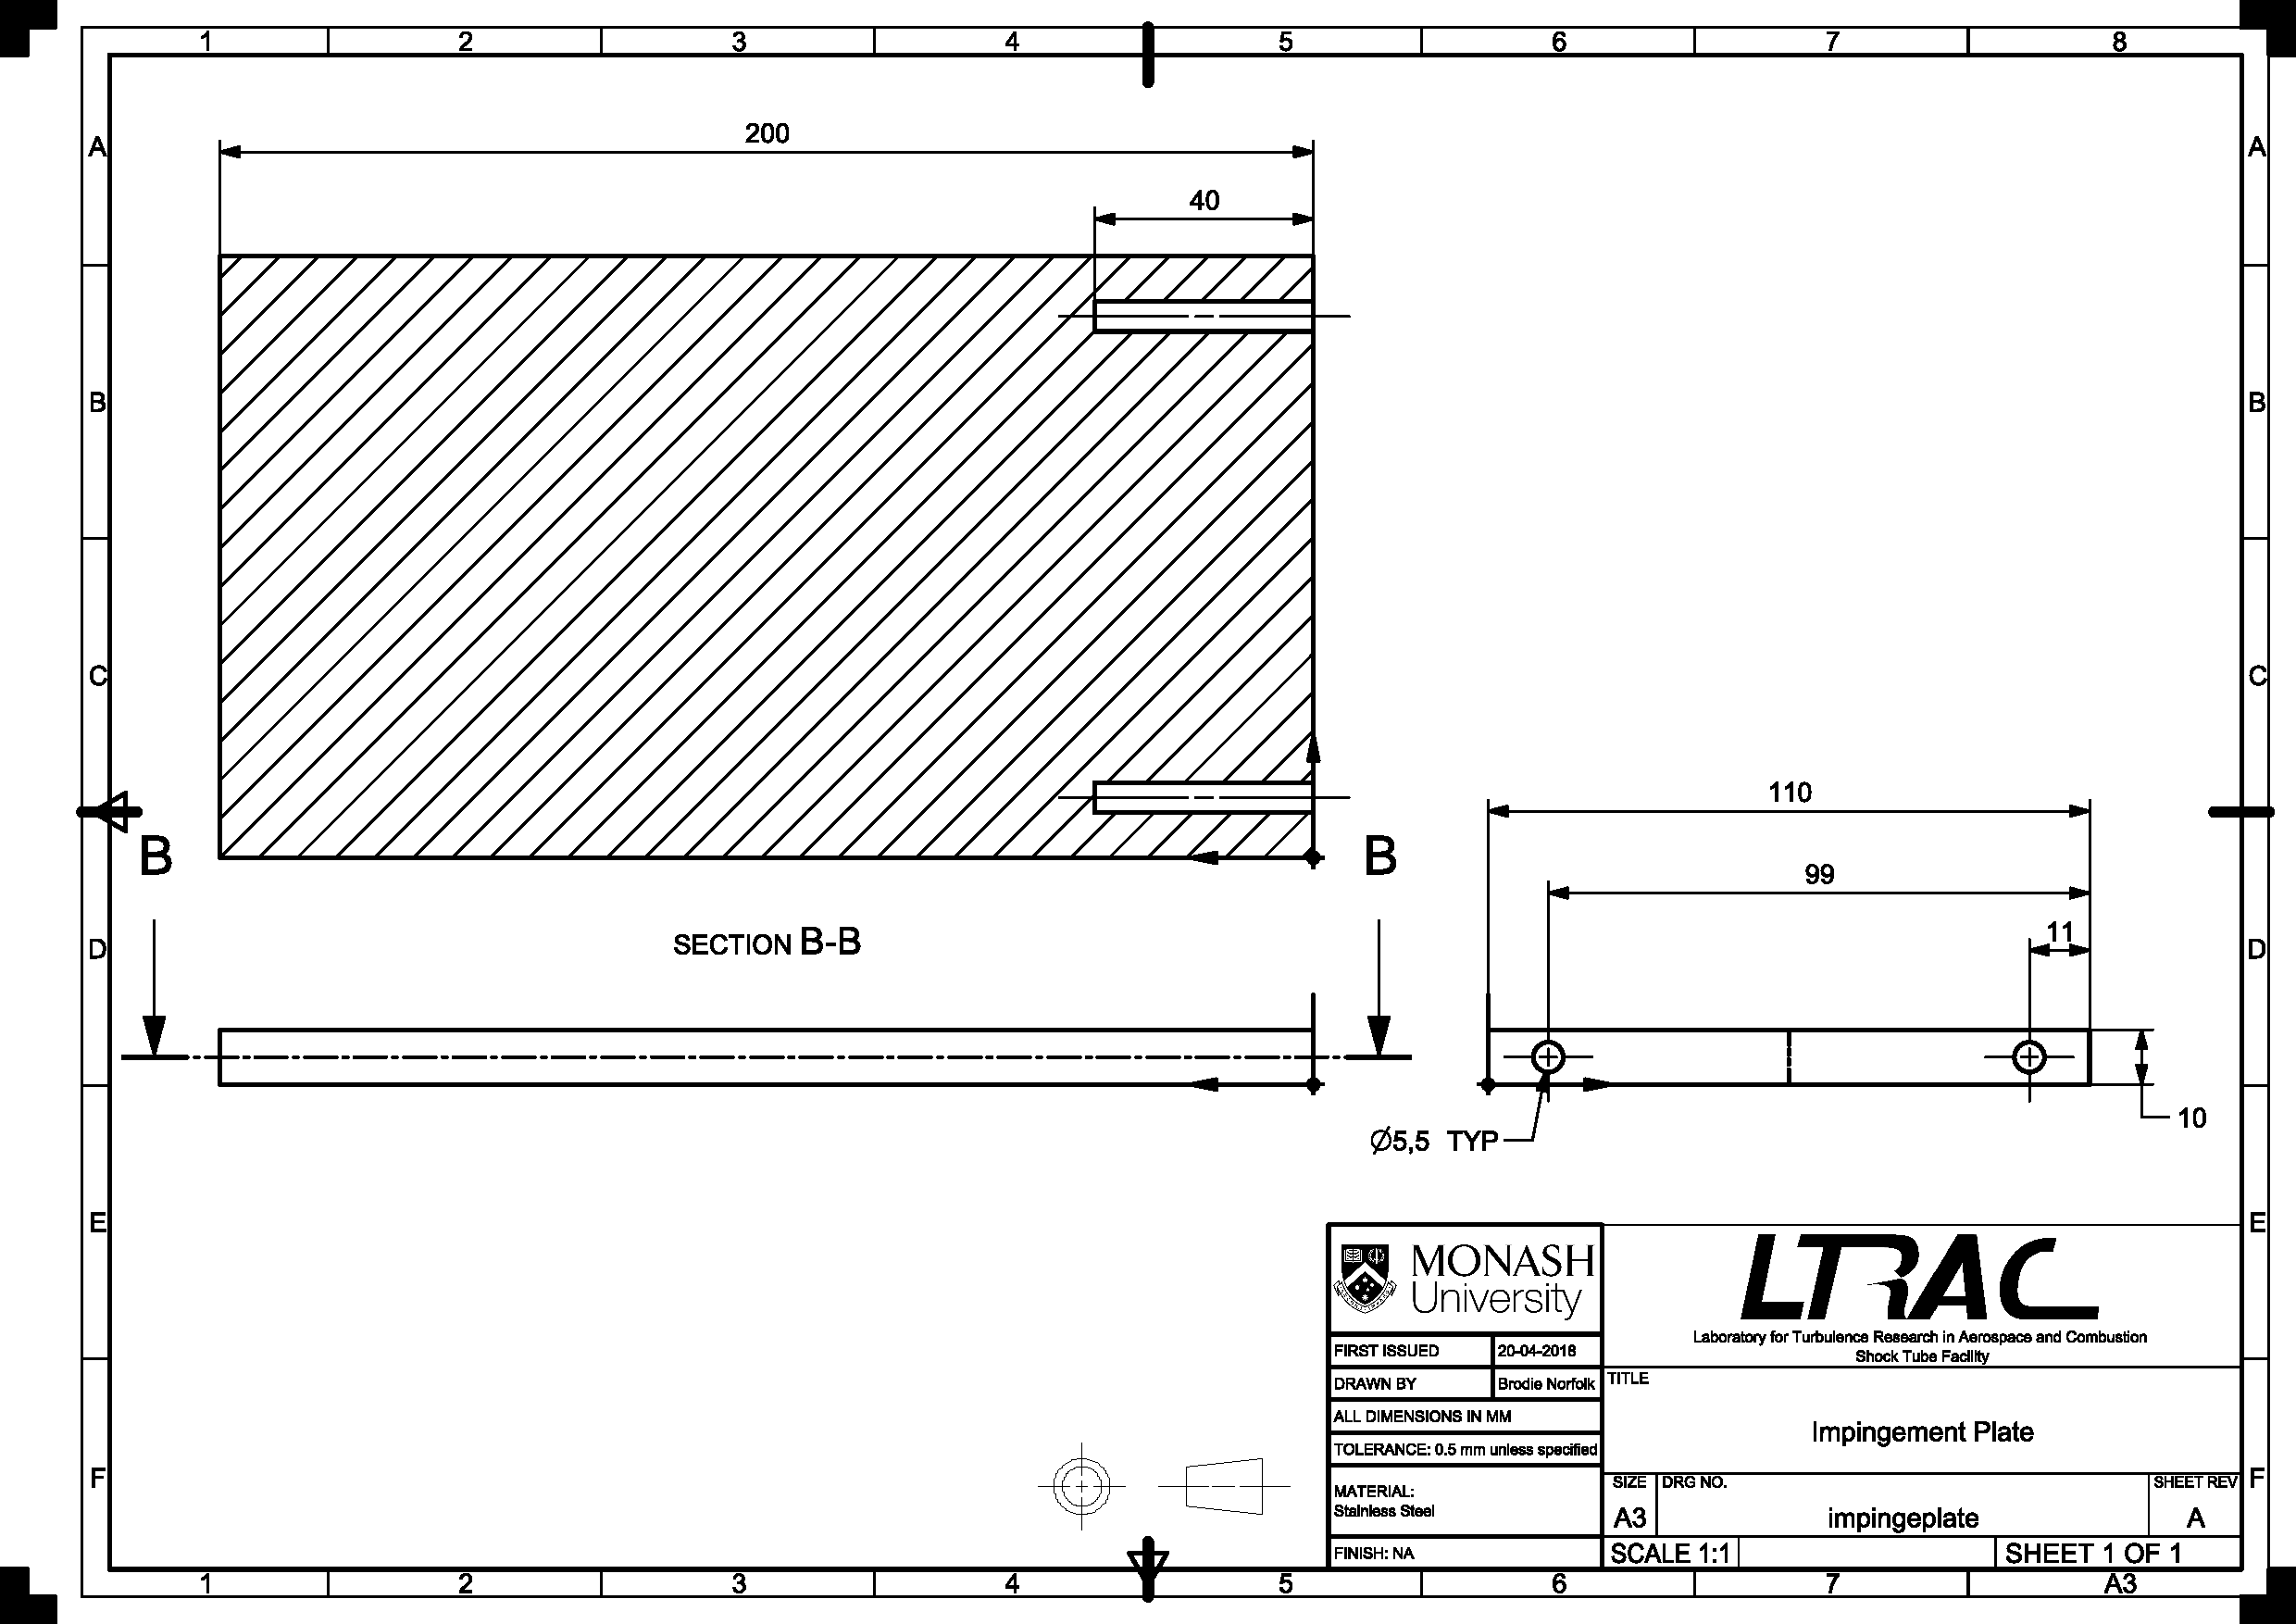
\includepdf[pages={-},fitpaper,pagecommand={}]{impingeplate.pdf}
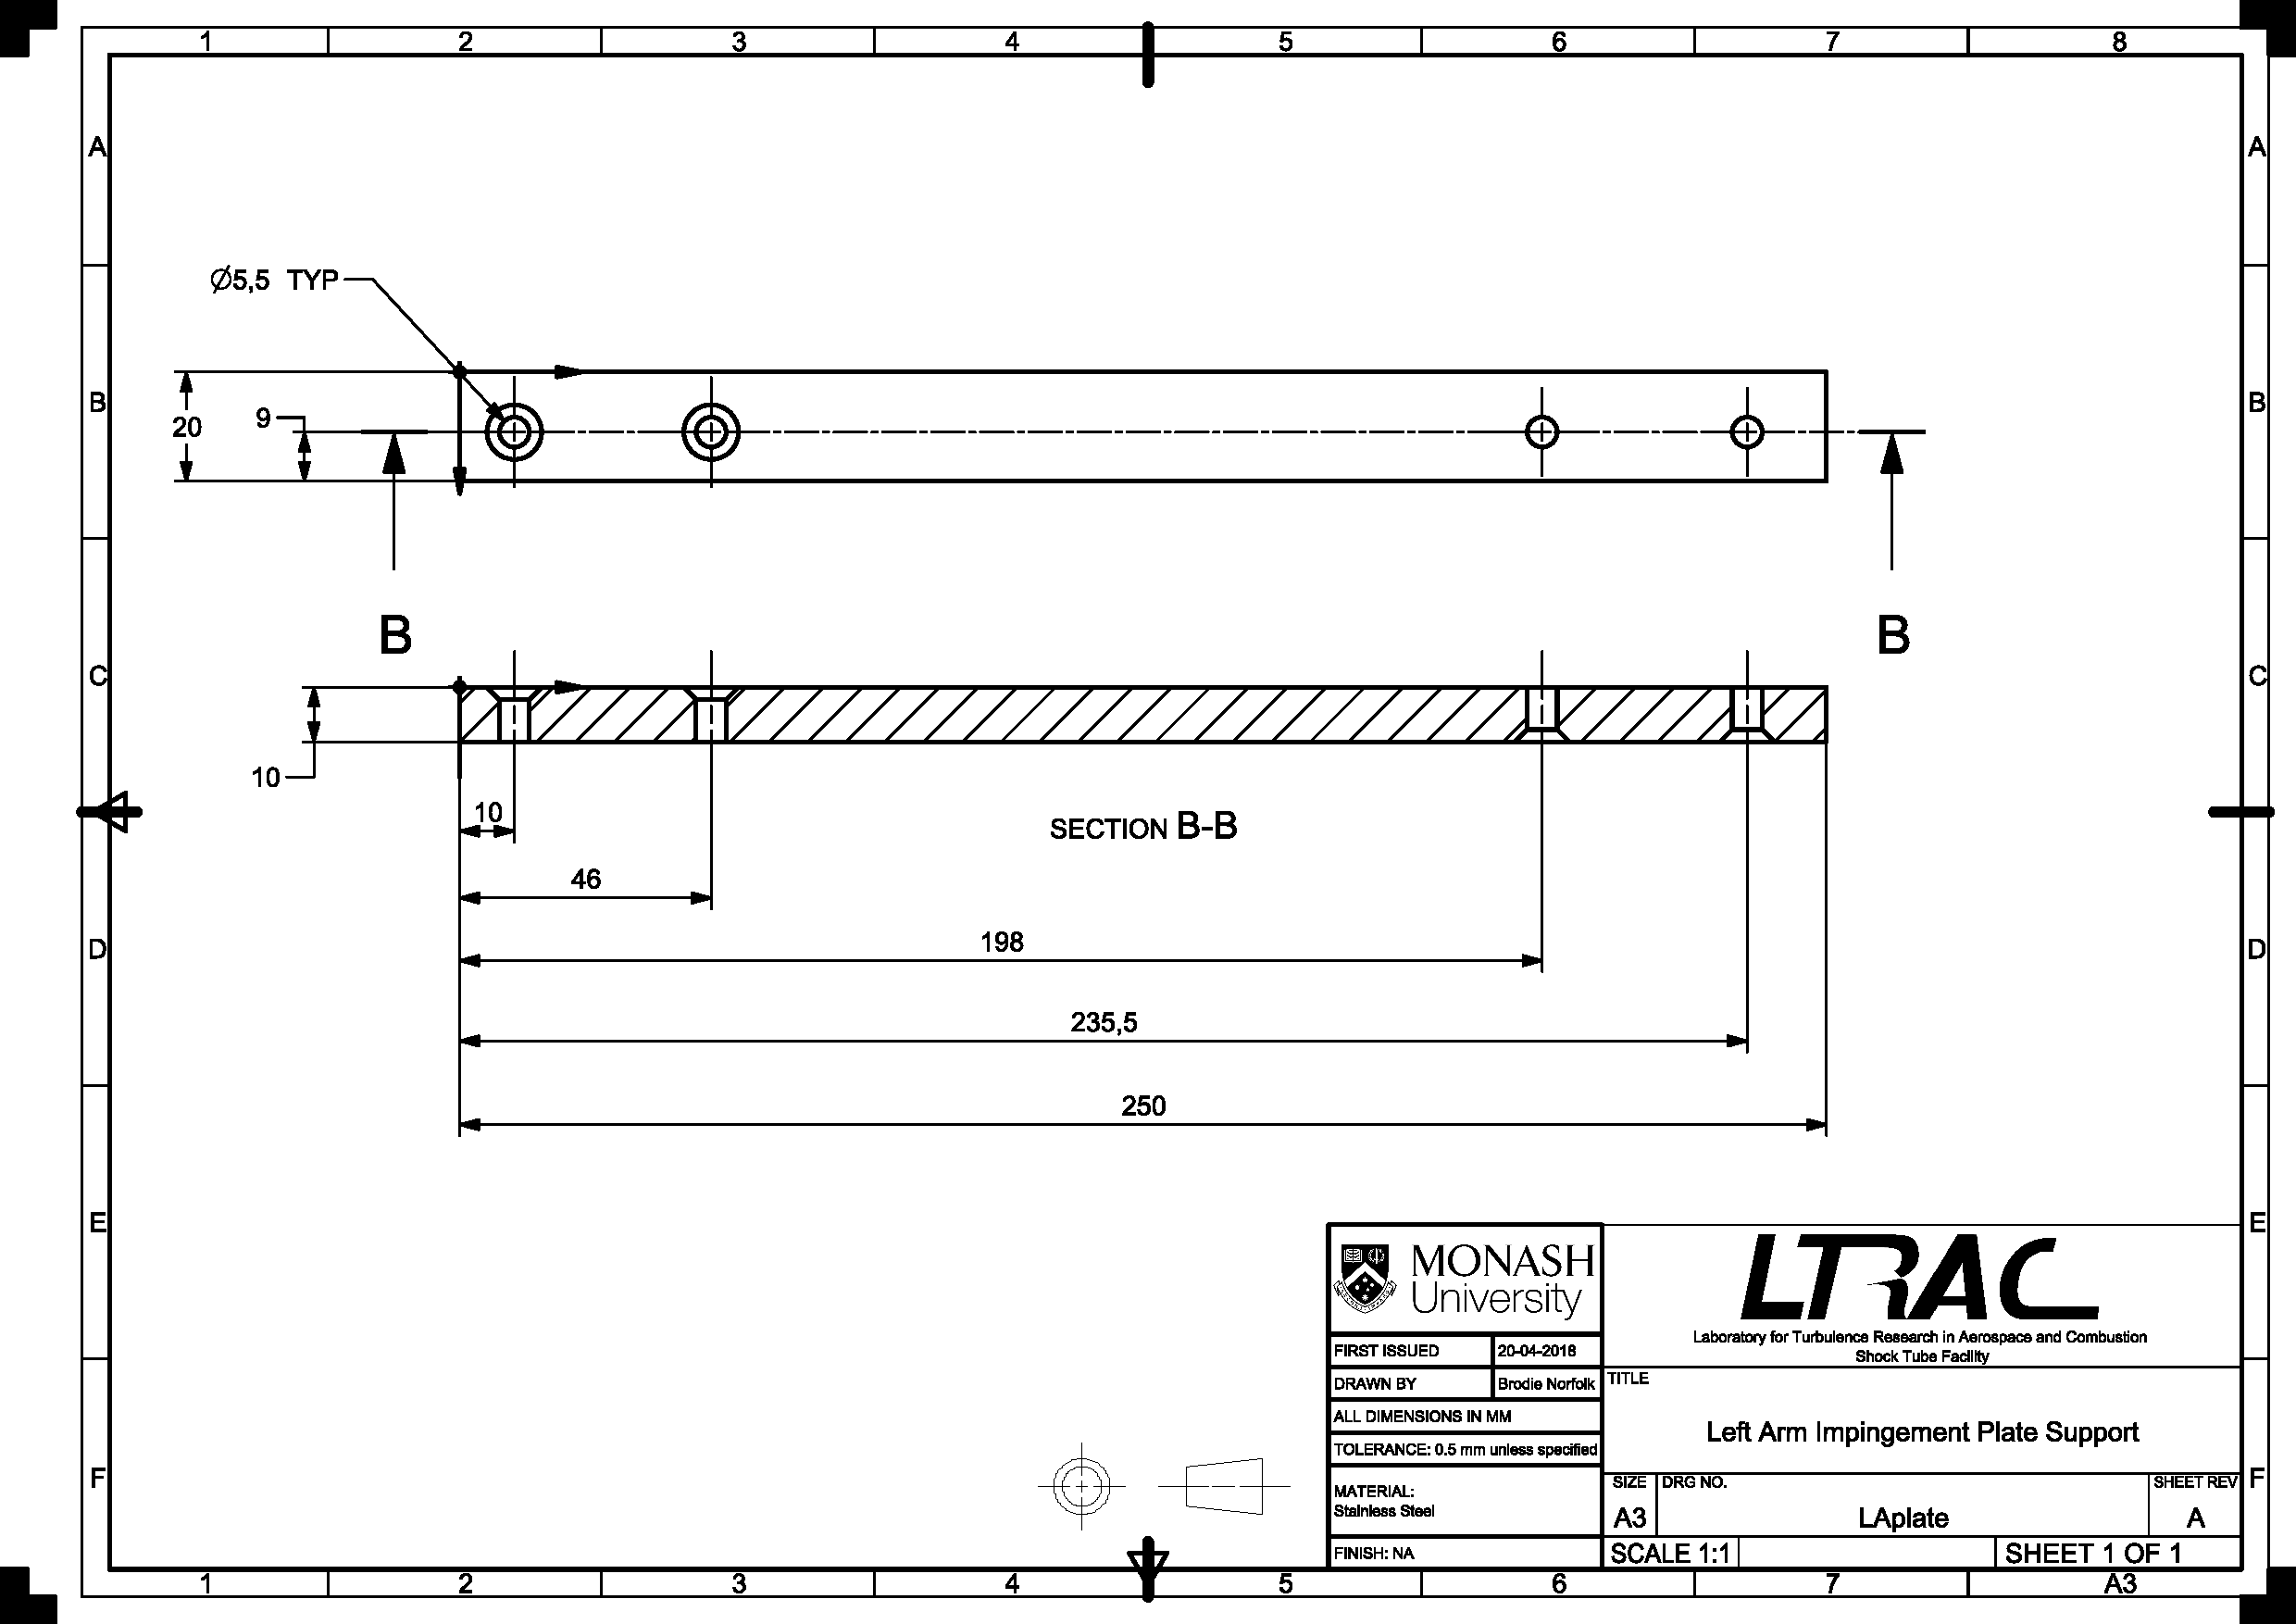
\includepdf[pages={-},fitpaper,pagecommand={}]{LAplate.pdf}
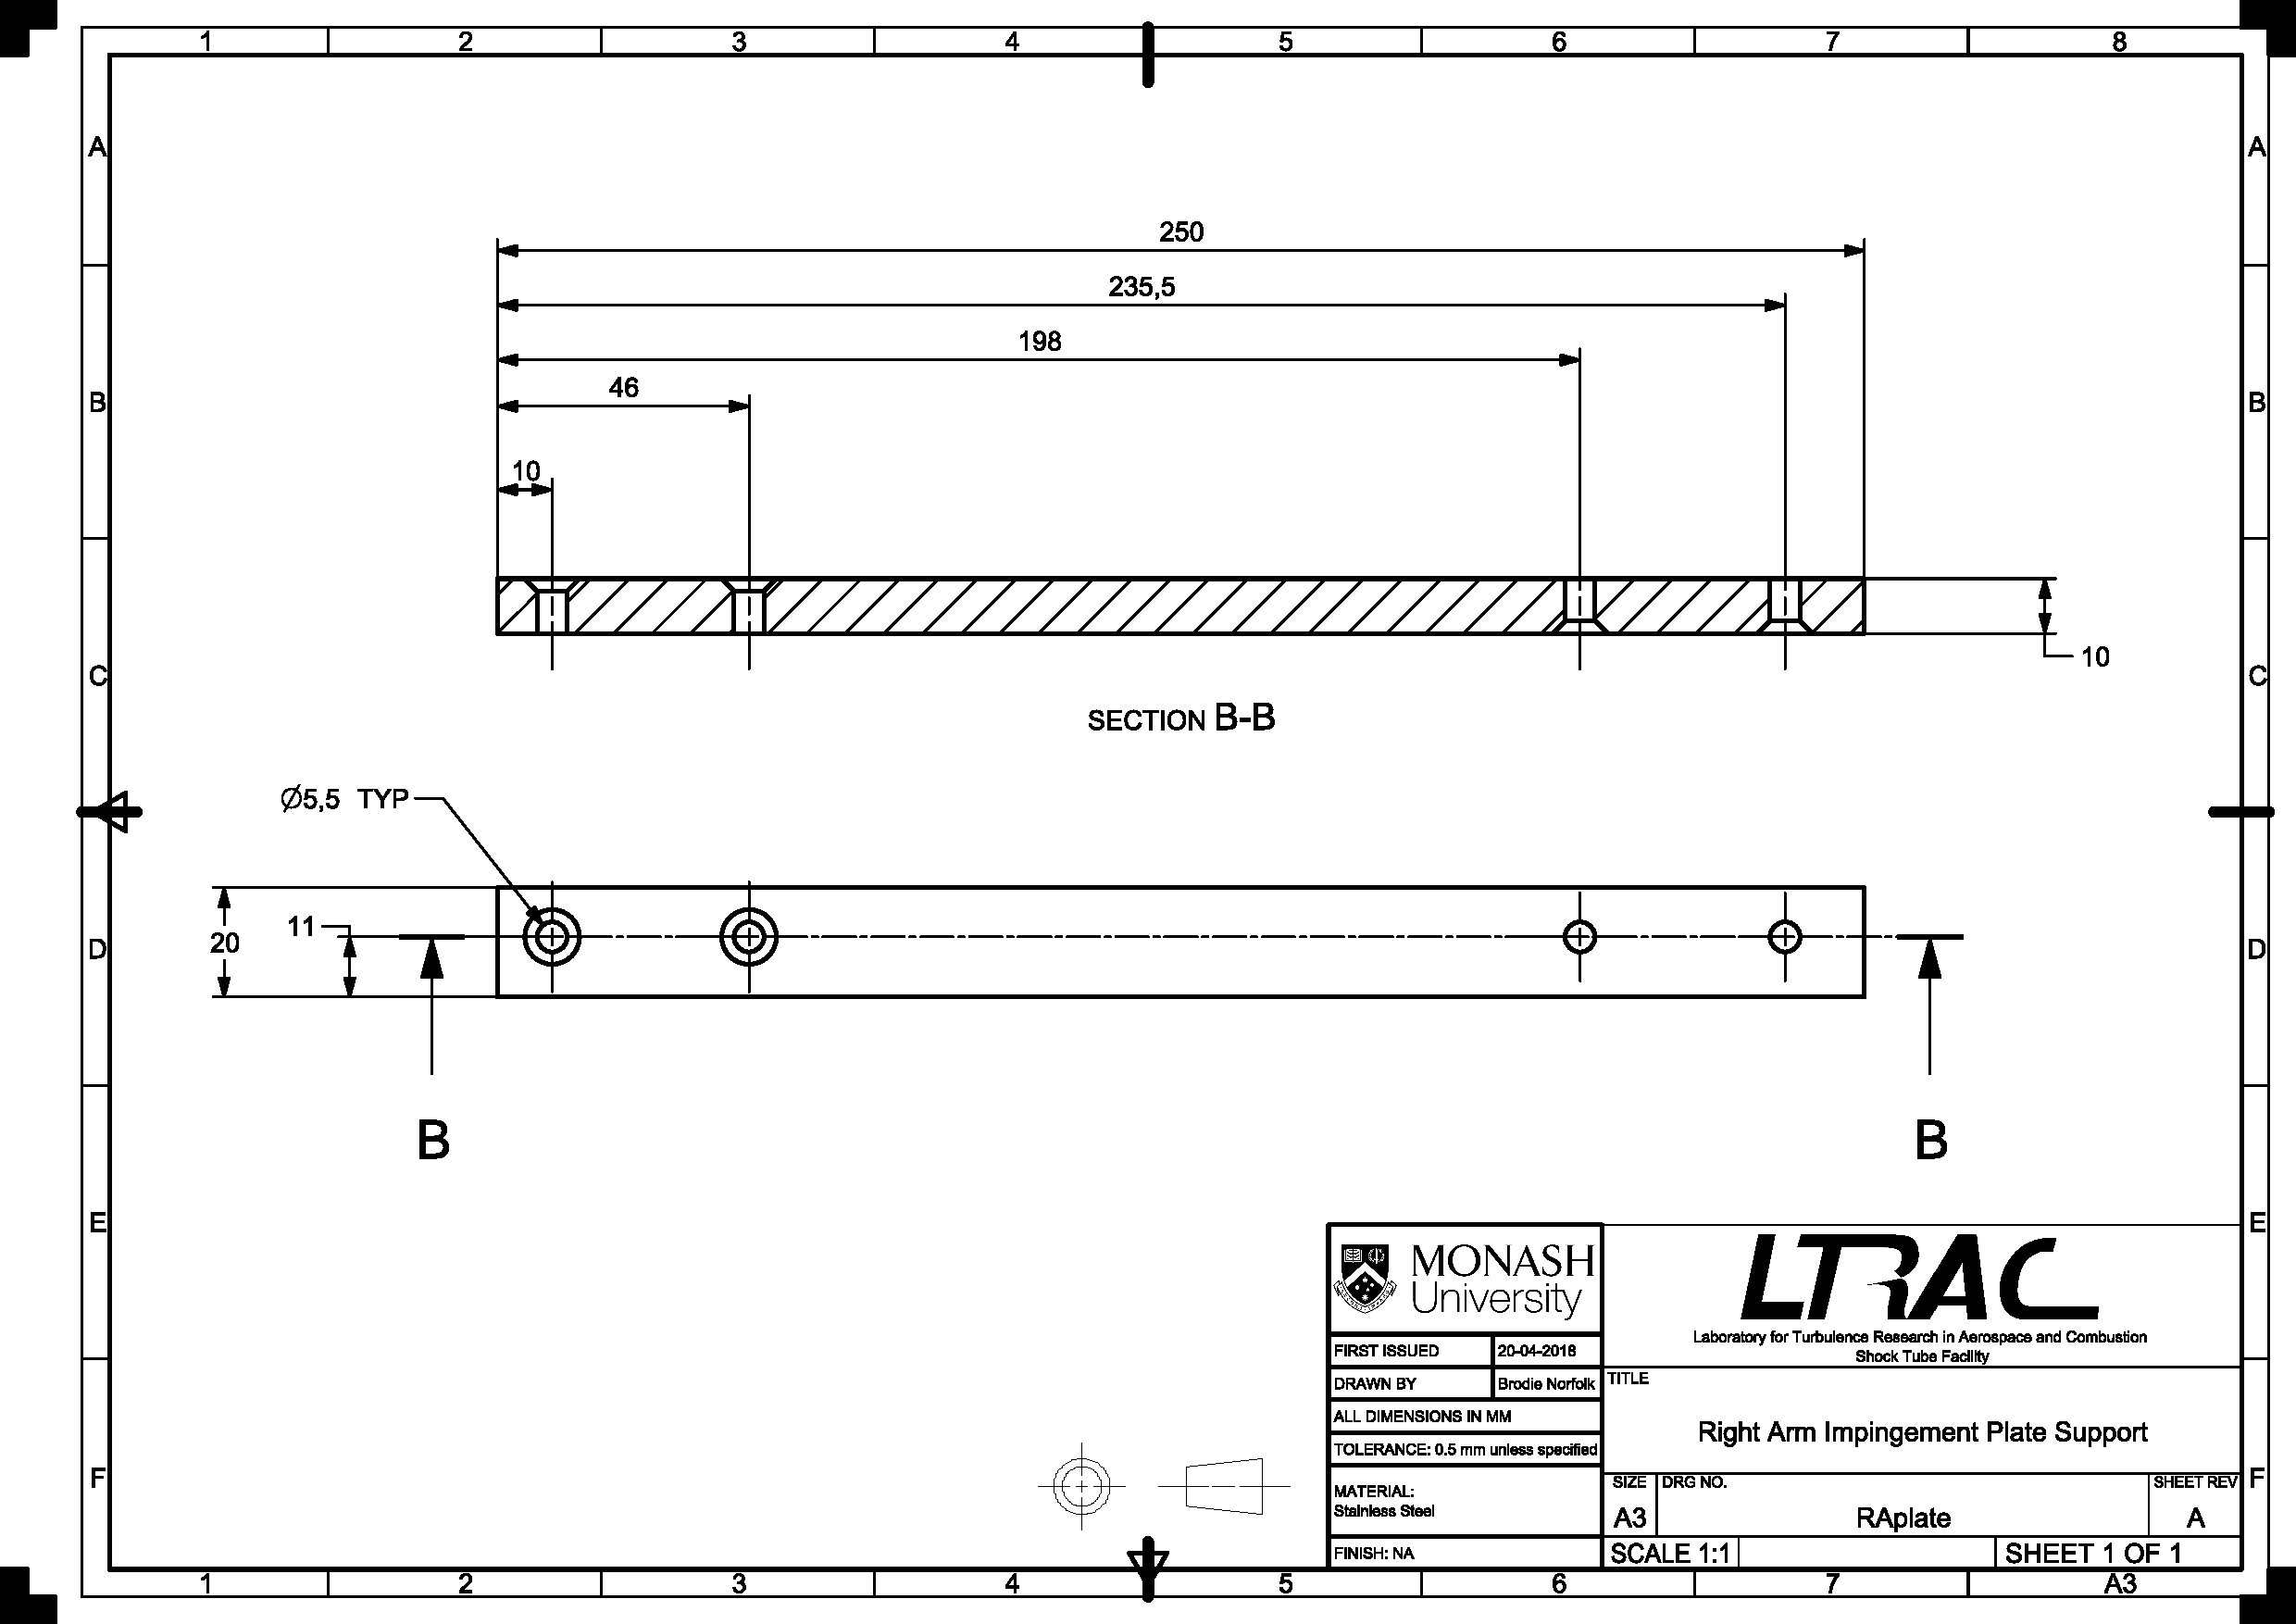
\includepdf[pages={-},fitpaper,pagecommand={}]{RAplate.pdf}
\section{Manufactured Components} \label{app:manufactured}

\begin{figure}[H] 
	\centering
	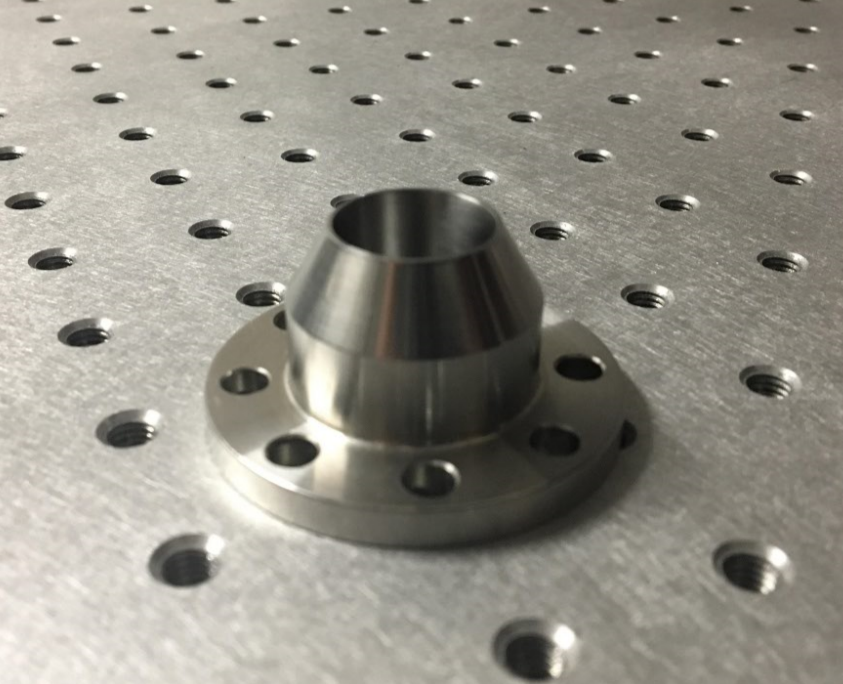
\includegraphics[scale=1.2]{fig11.PNG} 
	\caption{Diverging nozzle manufactured.}
	\label{fig:11}
\end{figure}

\begin{figure}[H] 
	\centering
	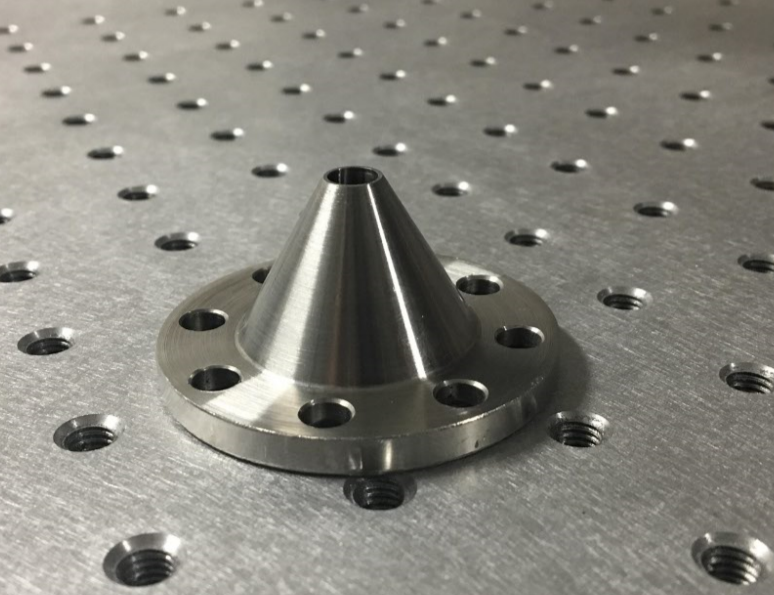
\includegraphics[scale=1.35]{fig12.PNG} 
	\caption{Converging nozzle manufactured.}
	\label{fig:12}
\end{figure}

\begin{figure}[H] 
	\centering
	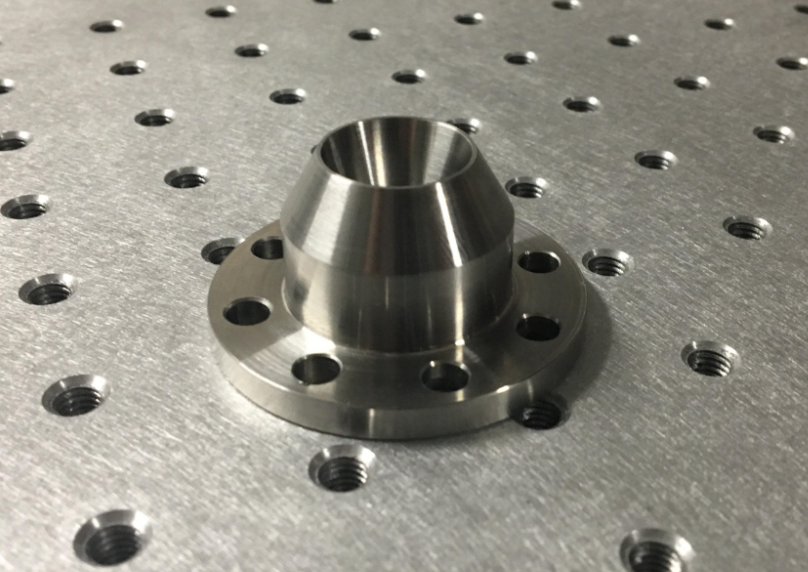
\includegraphics[scale=1.3]{fig13.PNG} 
	\caption{Converging-diverging nozzle manufactured.}
	\label{fig:13}
\end{figure}

\section{Previous Literature Results} \label{app:litresults}

\begin{figure}[H] 
	\centering
	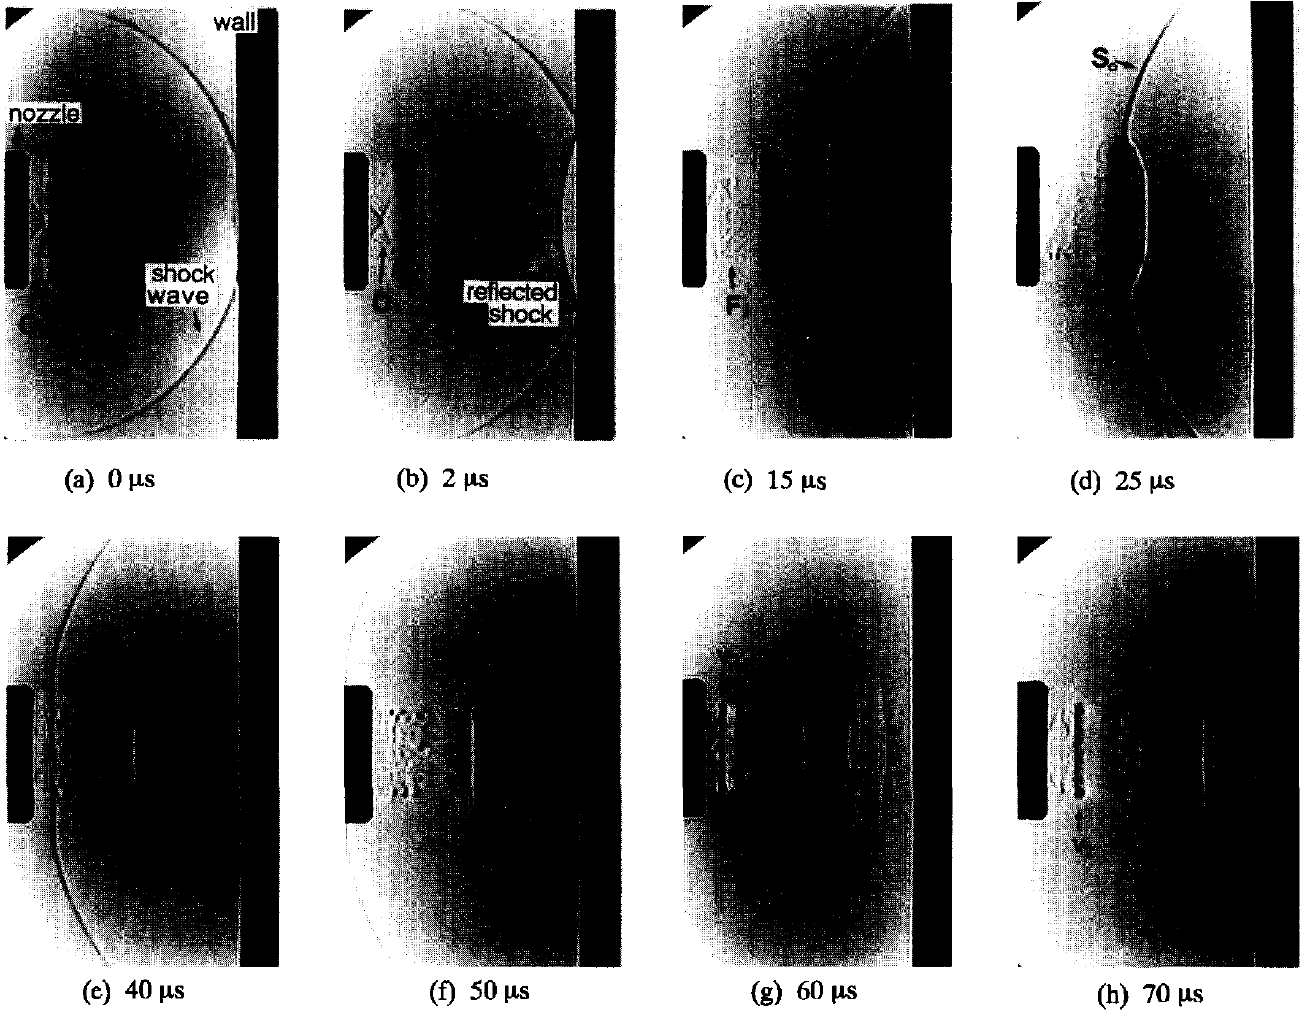
\includegraphics[scale=0.8]{minota.PNG} 
	\caption{\cite{minota1997}}
\end{figure}

\begin{figure}[H] 
	\centering
	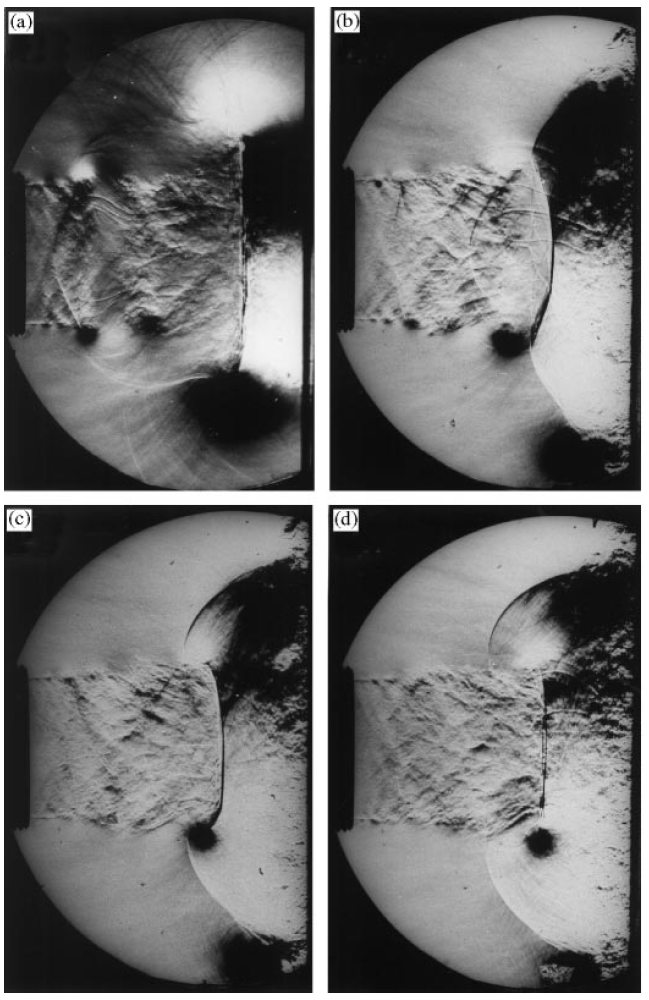
\includegraphics[scale=0.8]{szumowski.PNG} 
	\caption{\cite{szumowski2000}}
\end{figure}

\begin{figure}[H] 
	\centering
	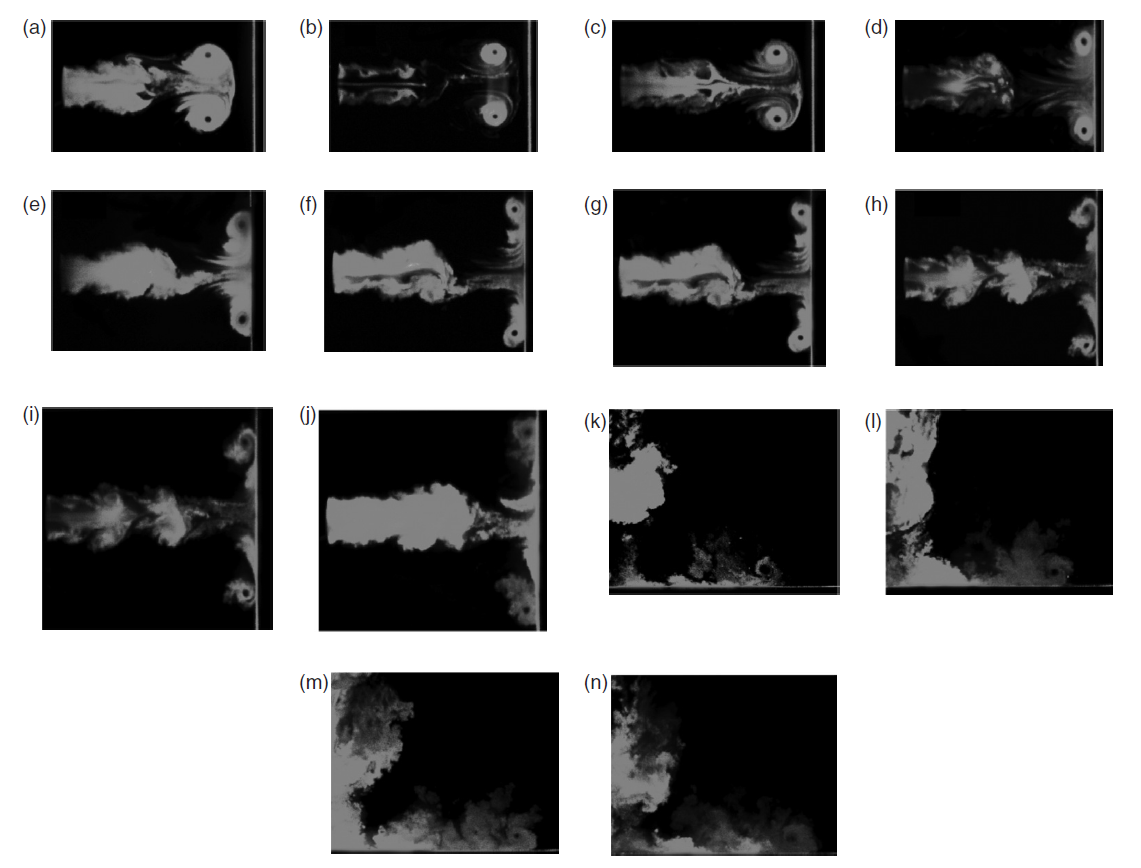
\includegraphics[width=\textwidth]{thangadurai2010.PNG} 
	\caption{\cite{murugan2010}}
\end{figure}

\begin{figure}[H] 
	\centering
	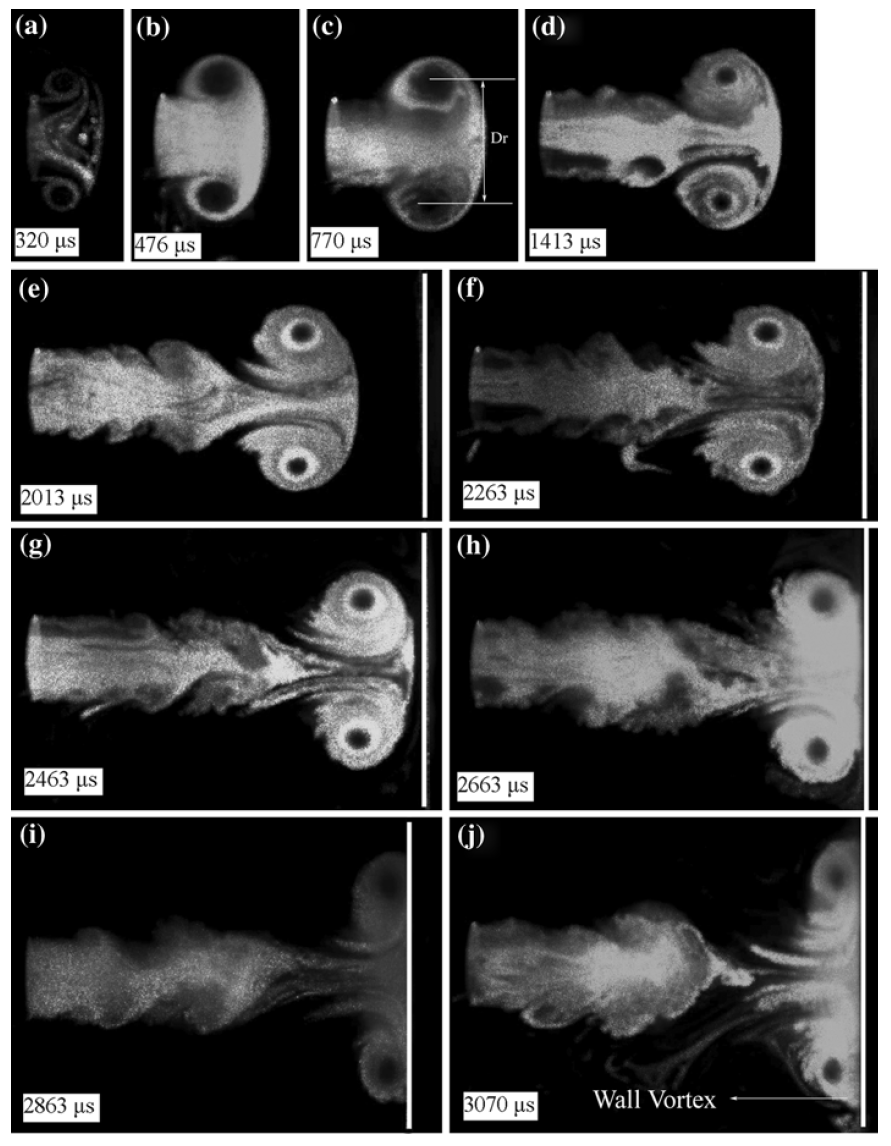
\includegraphics[scale=0.9]{thangadurai2012.PNG} 
	\caption{\cite{murugan2012}}
\end{figure}

\begin{figure}[H] 
	\centering
	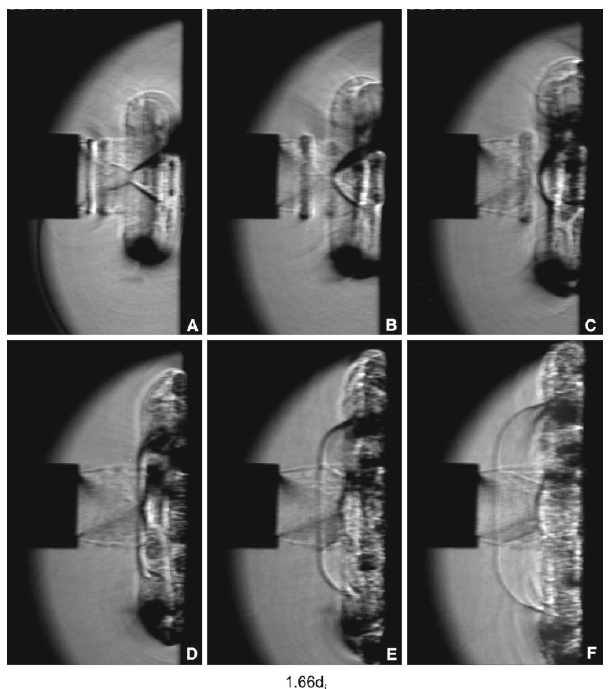
\includegraphics[scale=1.1]{mariani1.PNG} 
	\caption{\cite{mariani2013a}}
\end{figure}

\begin{figure}[H] 
	\centering
	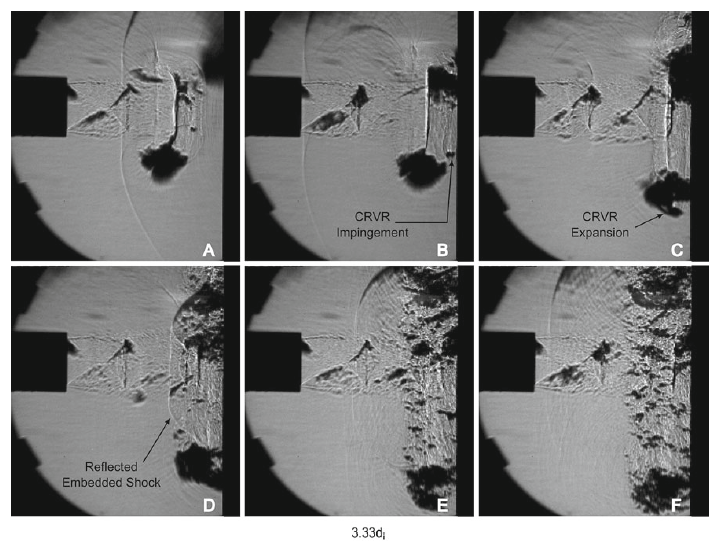
\includegraphics[width=0.9\textwidth]{mariani3.PNG} 
	\caption{\cite{mariani2013a}}
\end{figure}

\begin{figure}[h] 
	\centering
	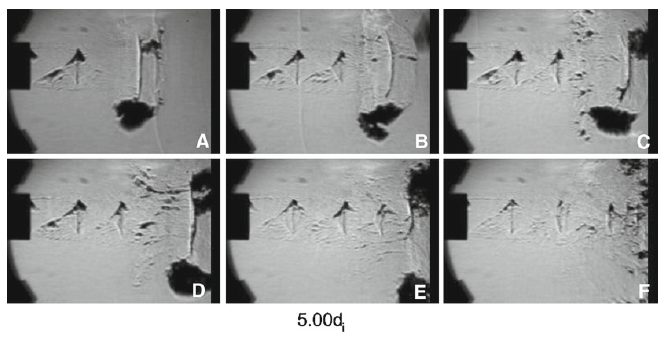
\includegraphics[width=0.9\textwidth]{mariani5.PNG} 
	\caption{\cite{mariani2013a}}
\end{figure}

\section{Saftey Documentation} \label{app:safety}

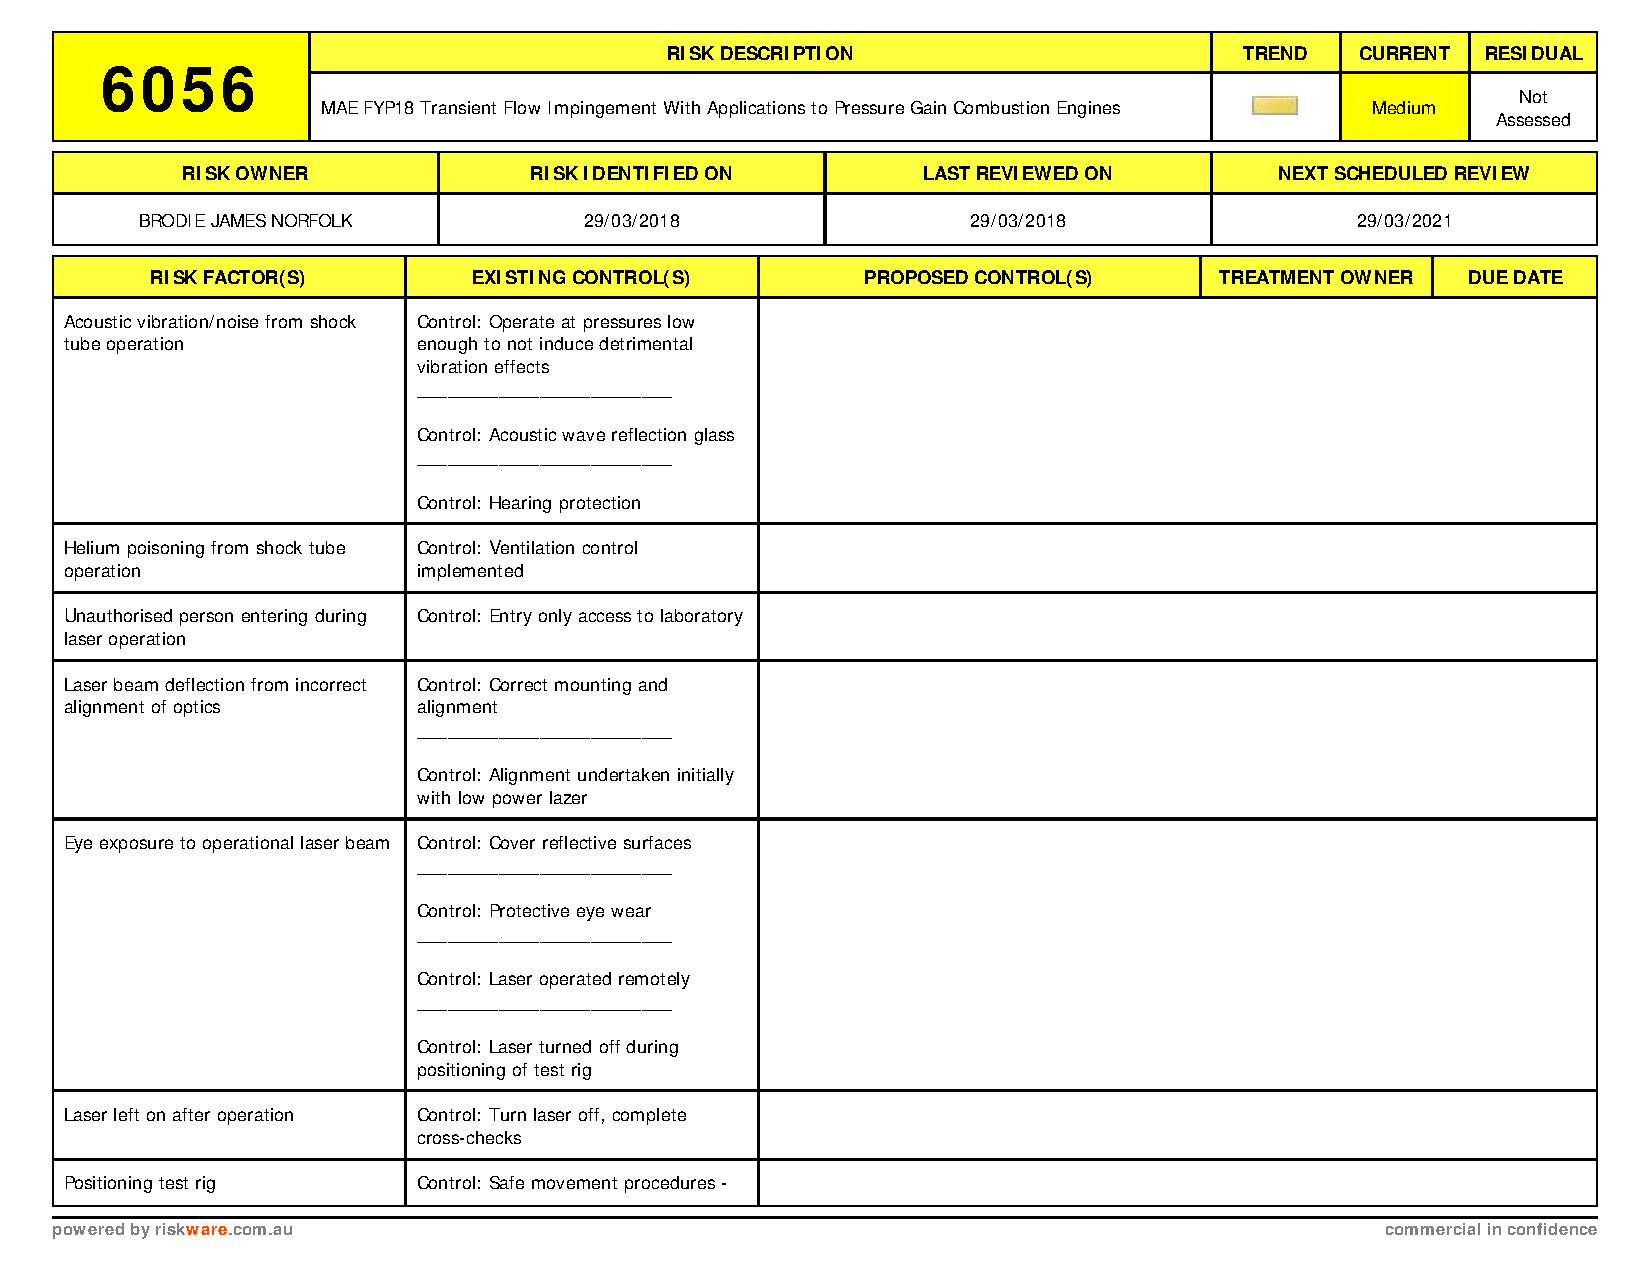
\includepdf[pages={-},fitpaper, pagecommand={}]{RiskOnAPage.pdf}

\section{Shock Relations} \label{app:shock}
In this section, the relationship between the pressure of the flow behind the leading shock and the ambient pressure will be derived. Figure \ref{fig:shock} details pressure, temperature, and velocity relations for the shock tube.
\begin{figure}[H]
	\centering
	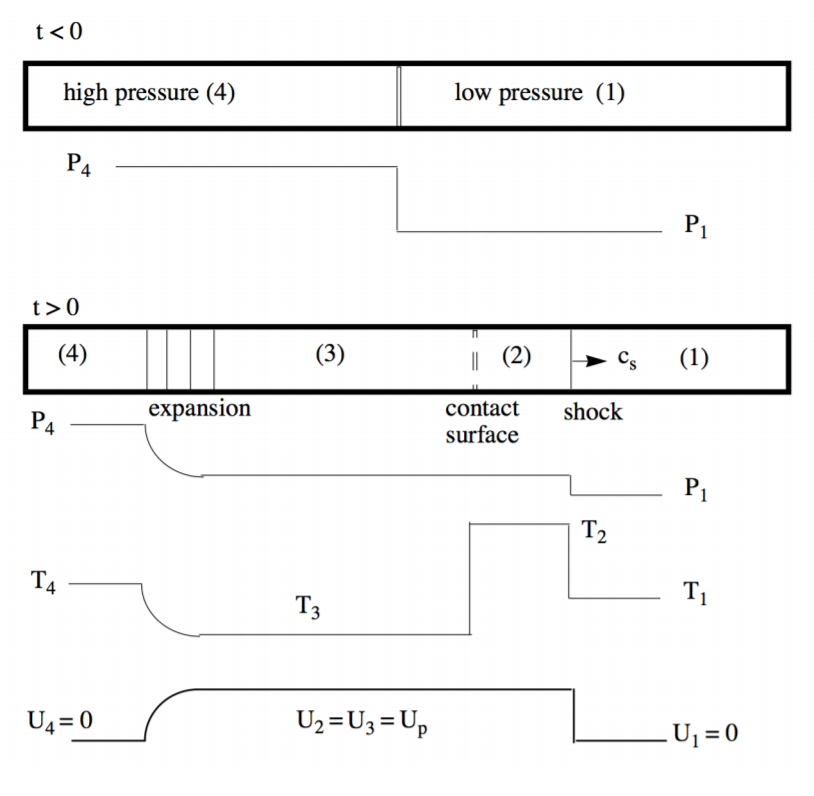
\includegraphics[scale=0.5]{figshock.png} 
	\caption{Shock tube flow regions: Region 1 is the flow ahead of the primary shock, region 2 is between contact surface and primary shock, region 3 is between tail of the expansion fan and contact surface, region 4 is ahead of the leading expansion wave.\cite{cantwell2017}}
	\label{fig:shock}
\end{figure}

In the following we will combine the results for expansion waves with normal shock relations to derive the so-called shock tube equation. The conditions at the contact surface are:
\begin{equation}
	P_2 = P_3 
\end{equation}
\begin{equation}
	U_2 = U_3 = U_p.
\end{equation}
\begin{center}
	where $U_2$ is the speed of the slug of gas set into motion by the opening of the diaphragm.
\end{center}
This is the effective piston speed of the fluid released by the diaphragm.

In a frame of reference moving with the shock wave the gas velocities are
\begin{equation}
U'_1 = -c_s
\end{equation}
\begin{equation}
U'_2 = -c_s + U_p
\end{equation}
and the shock jump conditions are

\begin{equation}
\frac{U'_2}{U'_1} = \frac{1+\frac{\gamma_1-1}{2}M_1^2}{\frac{\gamma_1+1}{2}M_1^2} 
\end{equation}
\begin{equation}
\frac{P_2}{P_1} = \frac{\gamma_1M_1^2-\frac{\gamma_1-1}{2}}{\frac{\gamma_1+1}{2}} 
\end{equation}
\begin{center}
	where $M_1 = c_s/a_1 = -U'_1/a_1$. Using the first relation, Equation 5 above, we can write
\end{center}

\begin{equation}
\frac{U'_2 - U'_1}{U'_1} = \frac{1 + \frac{\gamma_1-1}{2}M_1^2}{\frac{\gamma_1+1}{2}M_1^2} - 1 = \frac{1 - M_1^2}{\frac{\gamma_1+1}{2}M_1^2}
\end{equation}

The piston velocity is

\begin{equation}
U_p = U'_2 - U'_1 = U'_1\left(\frac{1 - M_1^2}{\frac{\gamma_1+1}{2}M_1\frac{-U'_1}{a_1}}\right) = a_1\left(\frac{M_1^2 - 1}{\frac{\gamma_1+1}{2}M_1}\right) 
\end{equation}

Note that $U_p$ is positive. Using the second relation, Equation 5, Equation 8 can be expressed in terms of the shock pressure ratio as 

\begin{equation}
U_p = a_1\left(\frac{P_2}{P_1} - 1\right)\left(\frac{2}{\gamma_1(\gamma_1 + 1)(P_2/P_1) + \gamma_1(\gamma_1 - 1)}\right)^{1/2}
\end{equation}

Equation 9 is the expression for the piston velocity derived using normal shock theory. Now lets work out an expression for the piston velocity using isentropic expansion theory. The velocity behind the expansion is

\begin{equation}
U_3 = U_p = \frac{2a_4}{\gamma_4 - 1}\left(1 - \frac{P_3}{P_4}^{\frac{\gamma_4 - 1}{2\gamma_4}}\right)
\end{equation}

Equate 9 and 10.

\begin{equation}
a_1\left(\frac{P_2}{P_1} - 1\right)\left(\frac{2}{\gamma_1(\gamma_1 + 1)(P_2/P_1) + \gamma_1(\gamma_1 - 1)}\right)^{1/2} = \frac{2a_4}{\gamma_4 - 1}\left(1 - \left(\frac{P_3}{P_2}\frac{P_2}{P_1}\frac{P_1}{P_4}\right)^{\frac{\gamma_4 - 1}{2\gamma_4}}\right)
\end{equation}

Using the following identity

\begin{equation}
\frac{P_3}{P_4}=\frac{P_3}{P_2}\frac{P_2}{P_1}\frac{P_1}{P_4}
\end{equation}

and noting that $P_3/P_2 = 1$ solve Equation 10 for $P_4/P_3 = 1$, substituting in $P_2/P_1$ from Equation 6. Simplifying, the result is the basic shock tube equation

\begin{equation}
\frac{P_4}{P_1} = \frac{2\gamma_1M_1^2 - (\gamma_1 - 1)}{\gamma_1 + 1}\left(1 - \frac{\gamma_{4-1}}{\gamma_{1+1}}\frac{U_1}{U_4}\left(M_1 - \frac{1}{M_1}\right)\right)^{-2\gamma_4/\gamma_{4-1}}
\end{equation}
And given the specific gas information, for the driver helium, $\gamma_4 = 1.667$, and the driven air, $\gamma_1 = 1.4$. Taking the ambient air temperature $T_1 = 273.15K$, the relation in equation 13 can be shown in the Figure \ref{fig:15}. This figure highlights the relationship between the driver pressure ratio at 4, and the ambient pressure at 1, for a design incident Mach number. The figure also illustrates the reduced pressure ratio benefit of using a helium to air experiment in comparison to a air to air experiment. 
	
\begin{figure}[H] 
	\centering
	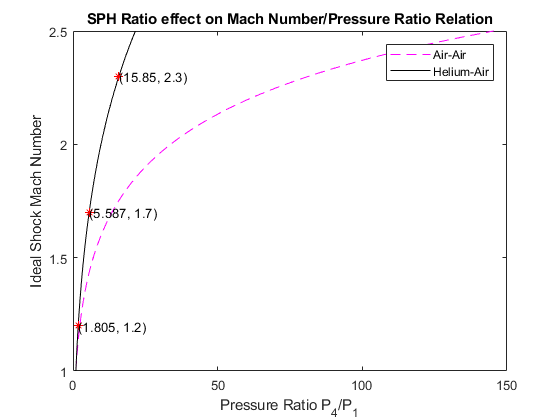
\includegraphics[scale=0.9]{fig1.png} 
	\caption{Specific Heat Capacity Ratio effect on Mach Number/Pressure Ratio.}
	\label{fig:15}
\end{figure}


\end{document}
